\documentclass[a4paper, 11pt]{article}
\usepackage[ngerman]{babel}
%ä und so
\usepackage[utf8]{inputenc}
\usepackage[T1]{fontenc}
\usepackage{amsmath}
\usepackage{amsthm}
\usepackage{amsbsy}

\usepackage{mathrsfs}
\usepackage{amssymb}
\usepackage{amstext}
\usepackage{amsfonts}
\usepackage{float}
\usepackage{graphicx}
\usepackage{esdiff}
\usepackage{hyperref}
\usepackage{geometry}
\geometry{top = 20mm, bottom = 20 mm, left = 25mm, right = 25mm}


\usepackage{setspace}
\onehalfspacing

\usepackage{fancyhdr}
\usepackage{wrapfig}
%\usepackage[hyphens]{url}
%\urlstyle{sf}
%\usepackage[hidelinks]{hyperref}
%\usepackage{breakurl}
%\hypersetup{colorlinks=false}
\usepackage{multirow}

%\usepackage{svg}

\title{Optik I $\looparrowright\rightsquigarrow\multimap$ Prismen- und Gitterspektroskopie}
\author{Gruppe B14 \\ \\ Daniel Wendland \\ Philipp Bremer \\ Olexiy Fedorets \\ Jonathan Hermann}
\date{\today}

% !TeX spellcheck = de_DE
\begin{document}


\begin{titlepage}
	\vspace*{\fill}
	\begin{center}
		\vskip -0.25\textheight
		\vfill
		\newcommand{\Line}{\rule{\linewidth}{0.6mm}}
		\Line 
		{\let\newpage\relax\maketitle}
		\Line 
		\vfill
	\end{center}
	
	%\begin{figure}[H]
	%	\begin{minipage}[h]{0.2\textwidth}
	%	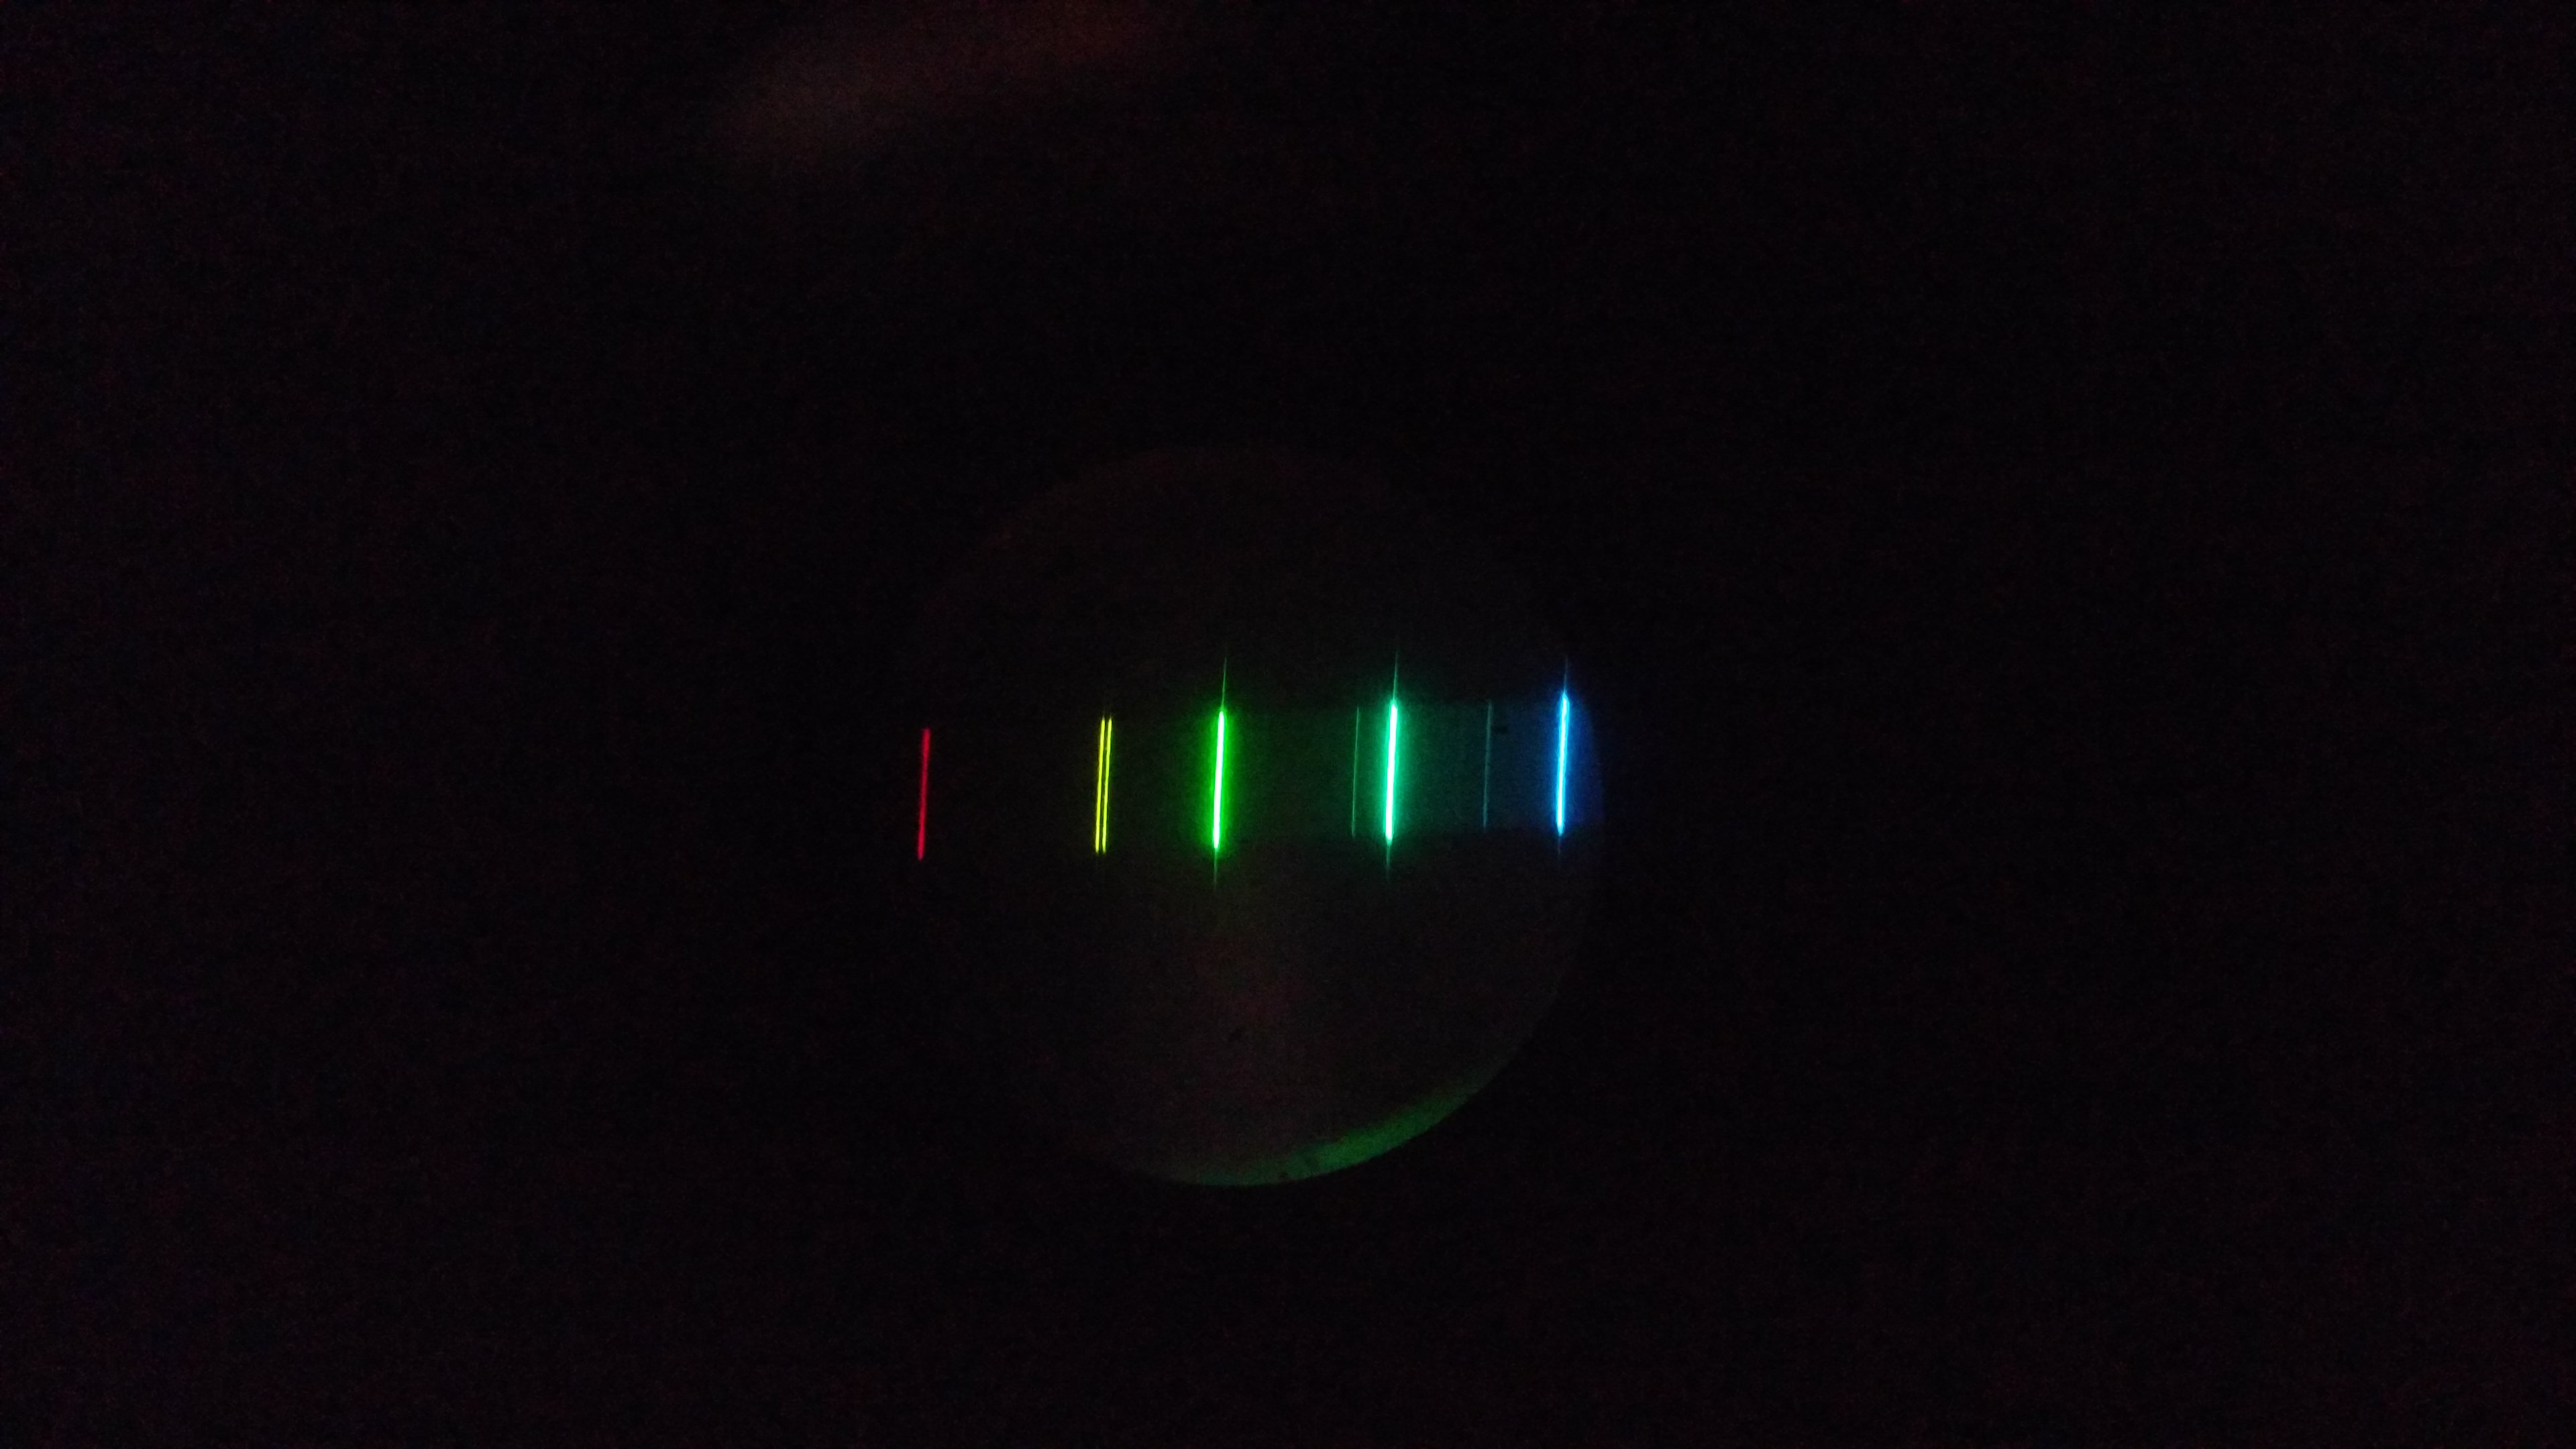
\includegraphics[scale=0.08]{Bilder/IMG_20170915_131423.jpg}  
	%	\end{minipage}
	%	\hspace{0.15\textwidth}
	%	\begin{minipage}[h]{0.2\textwidth}
	%	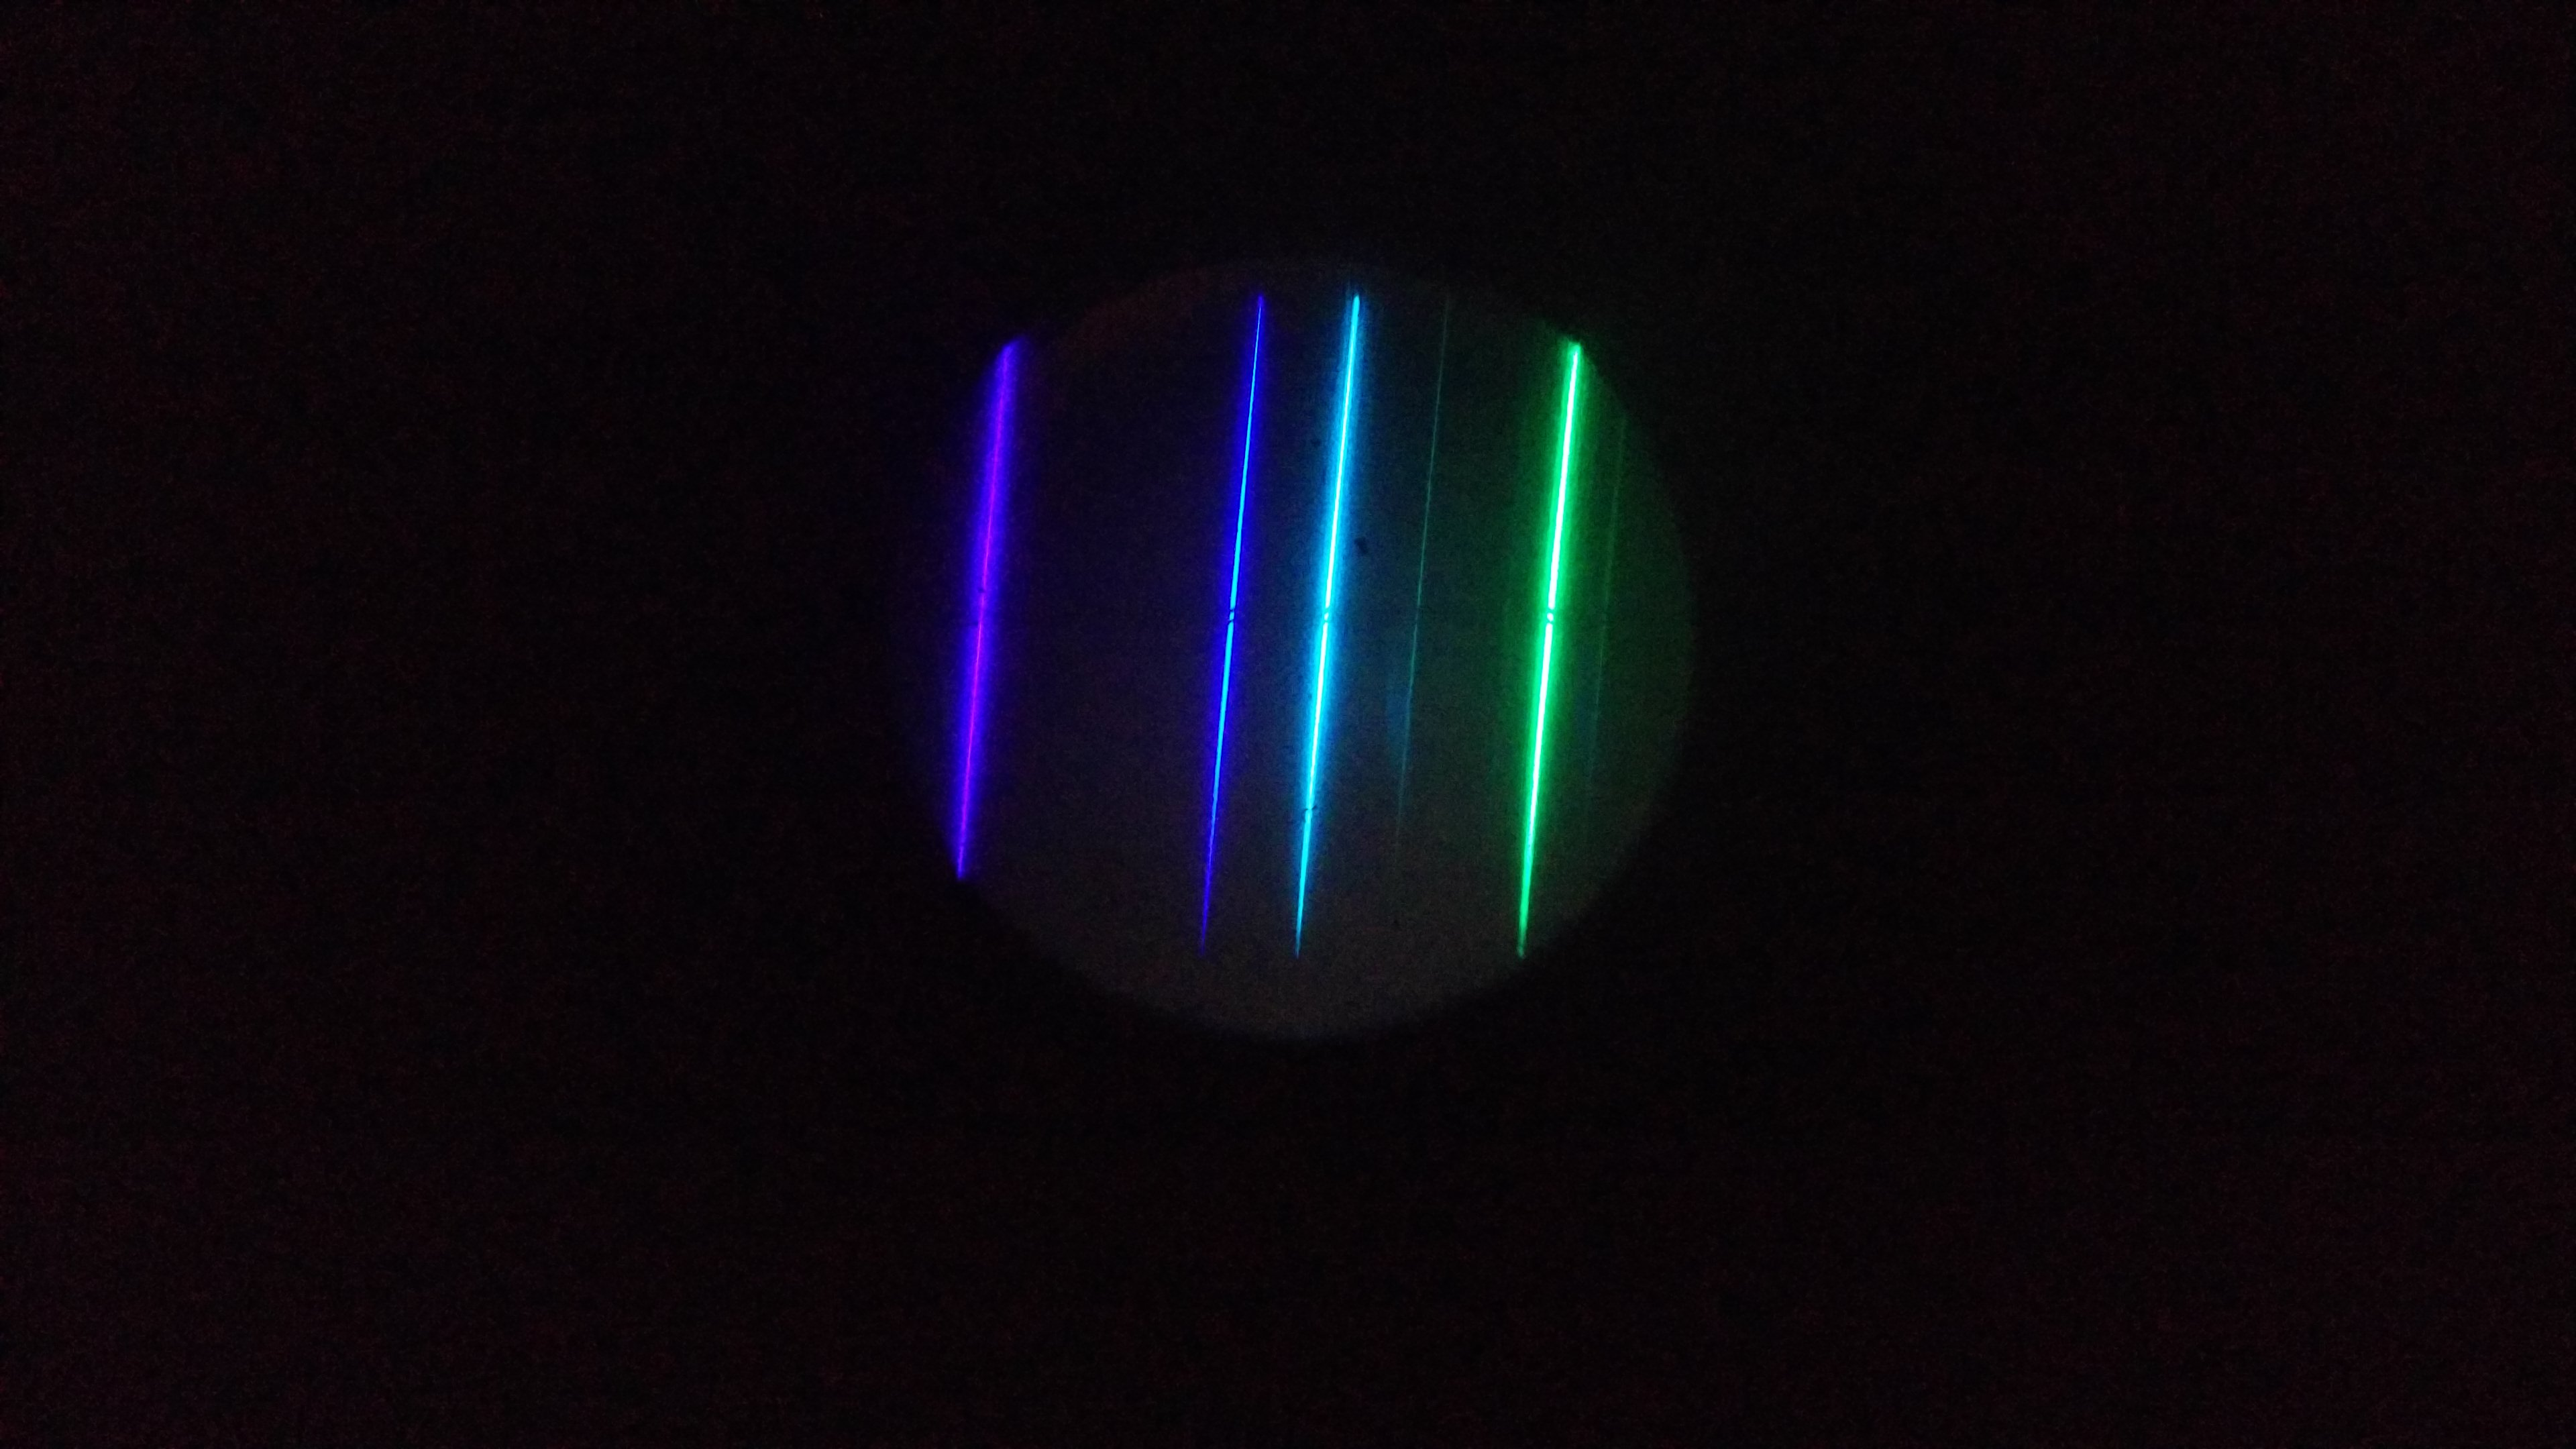
\includegraphics[scale=0.08]{Bilder/IMG_20170915_131047.jpg}  
	%	\end{minipage}
	%\end{figure}
	
	\begin{center}
		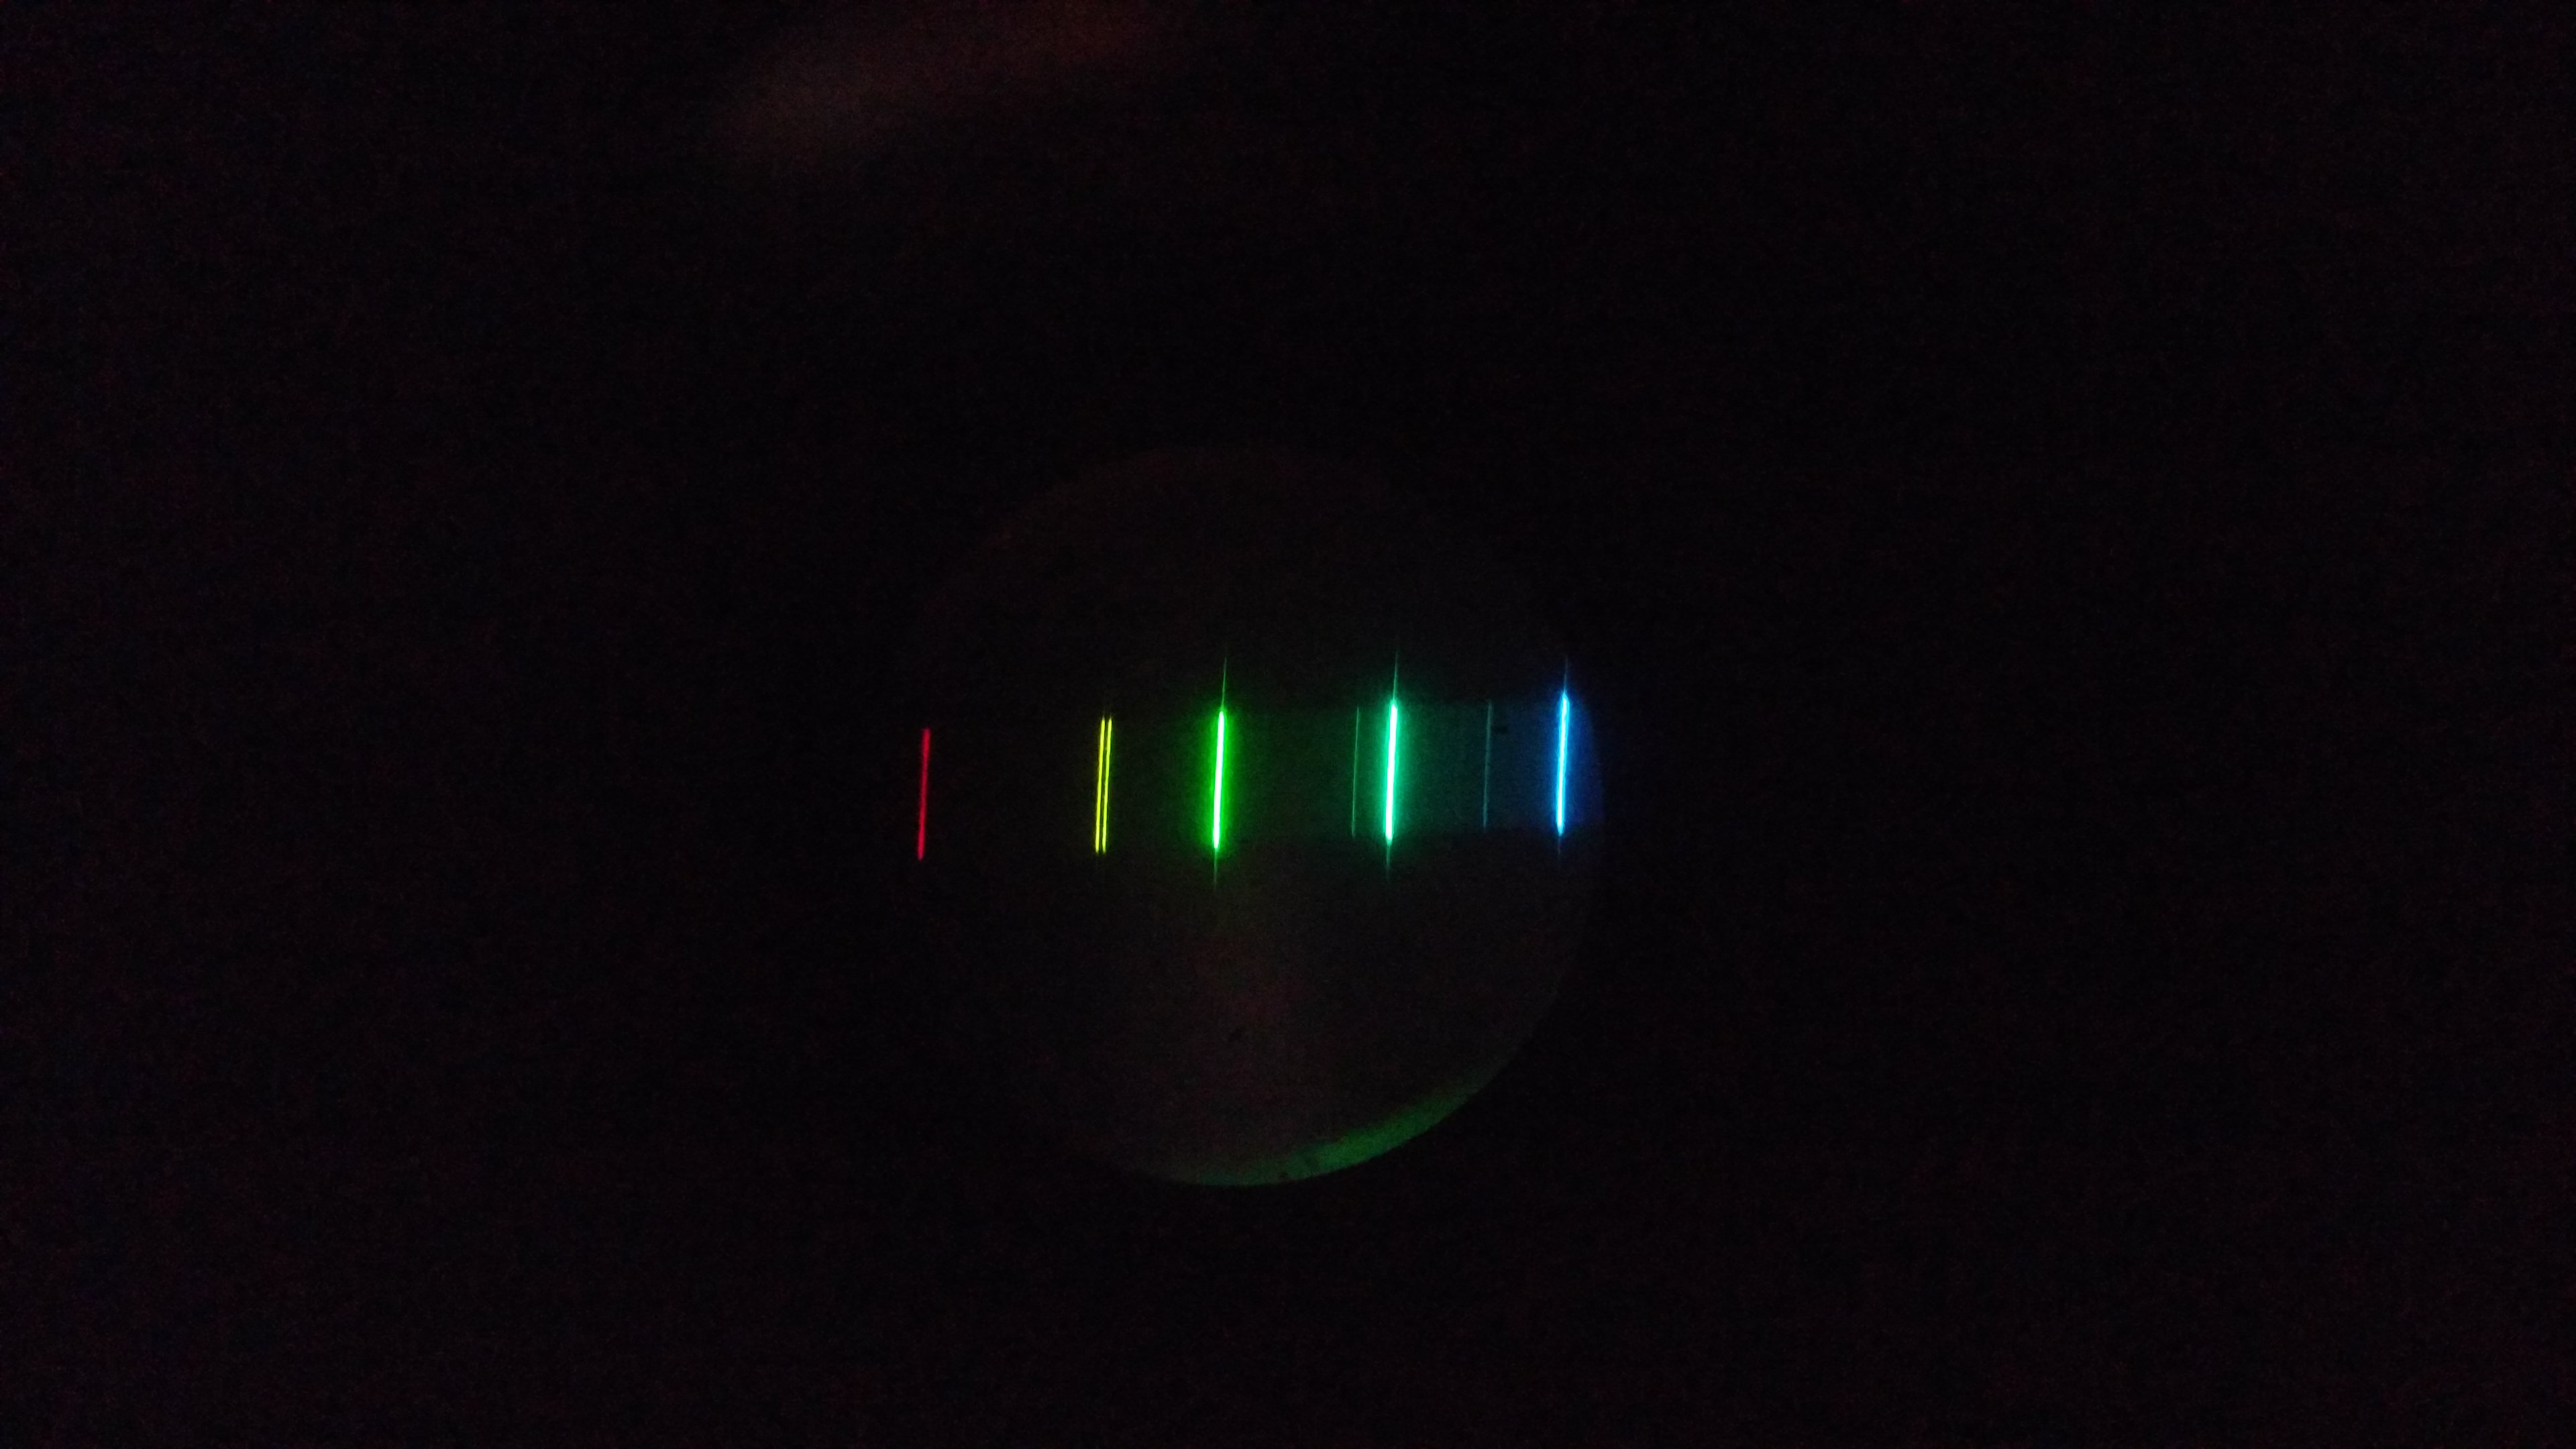
\includegraphics[trim={1cm 1cm 1cm 1cm},clip=true,scale=0.08]{Bilder/IMG_20170915_131423.jpg}  
		\vskip -0.07\textwidth
		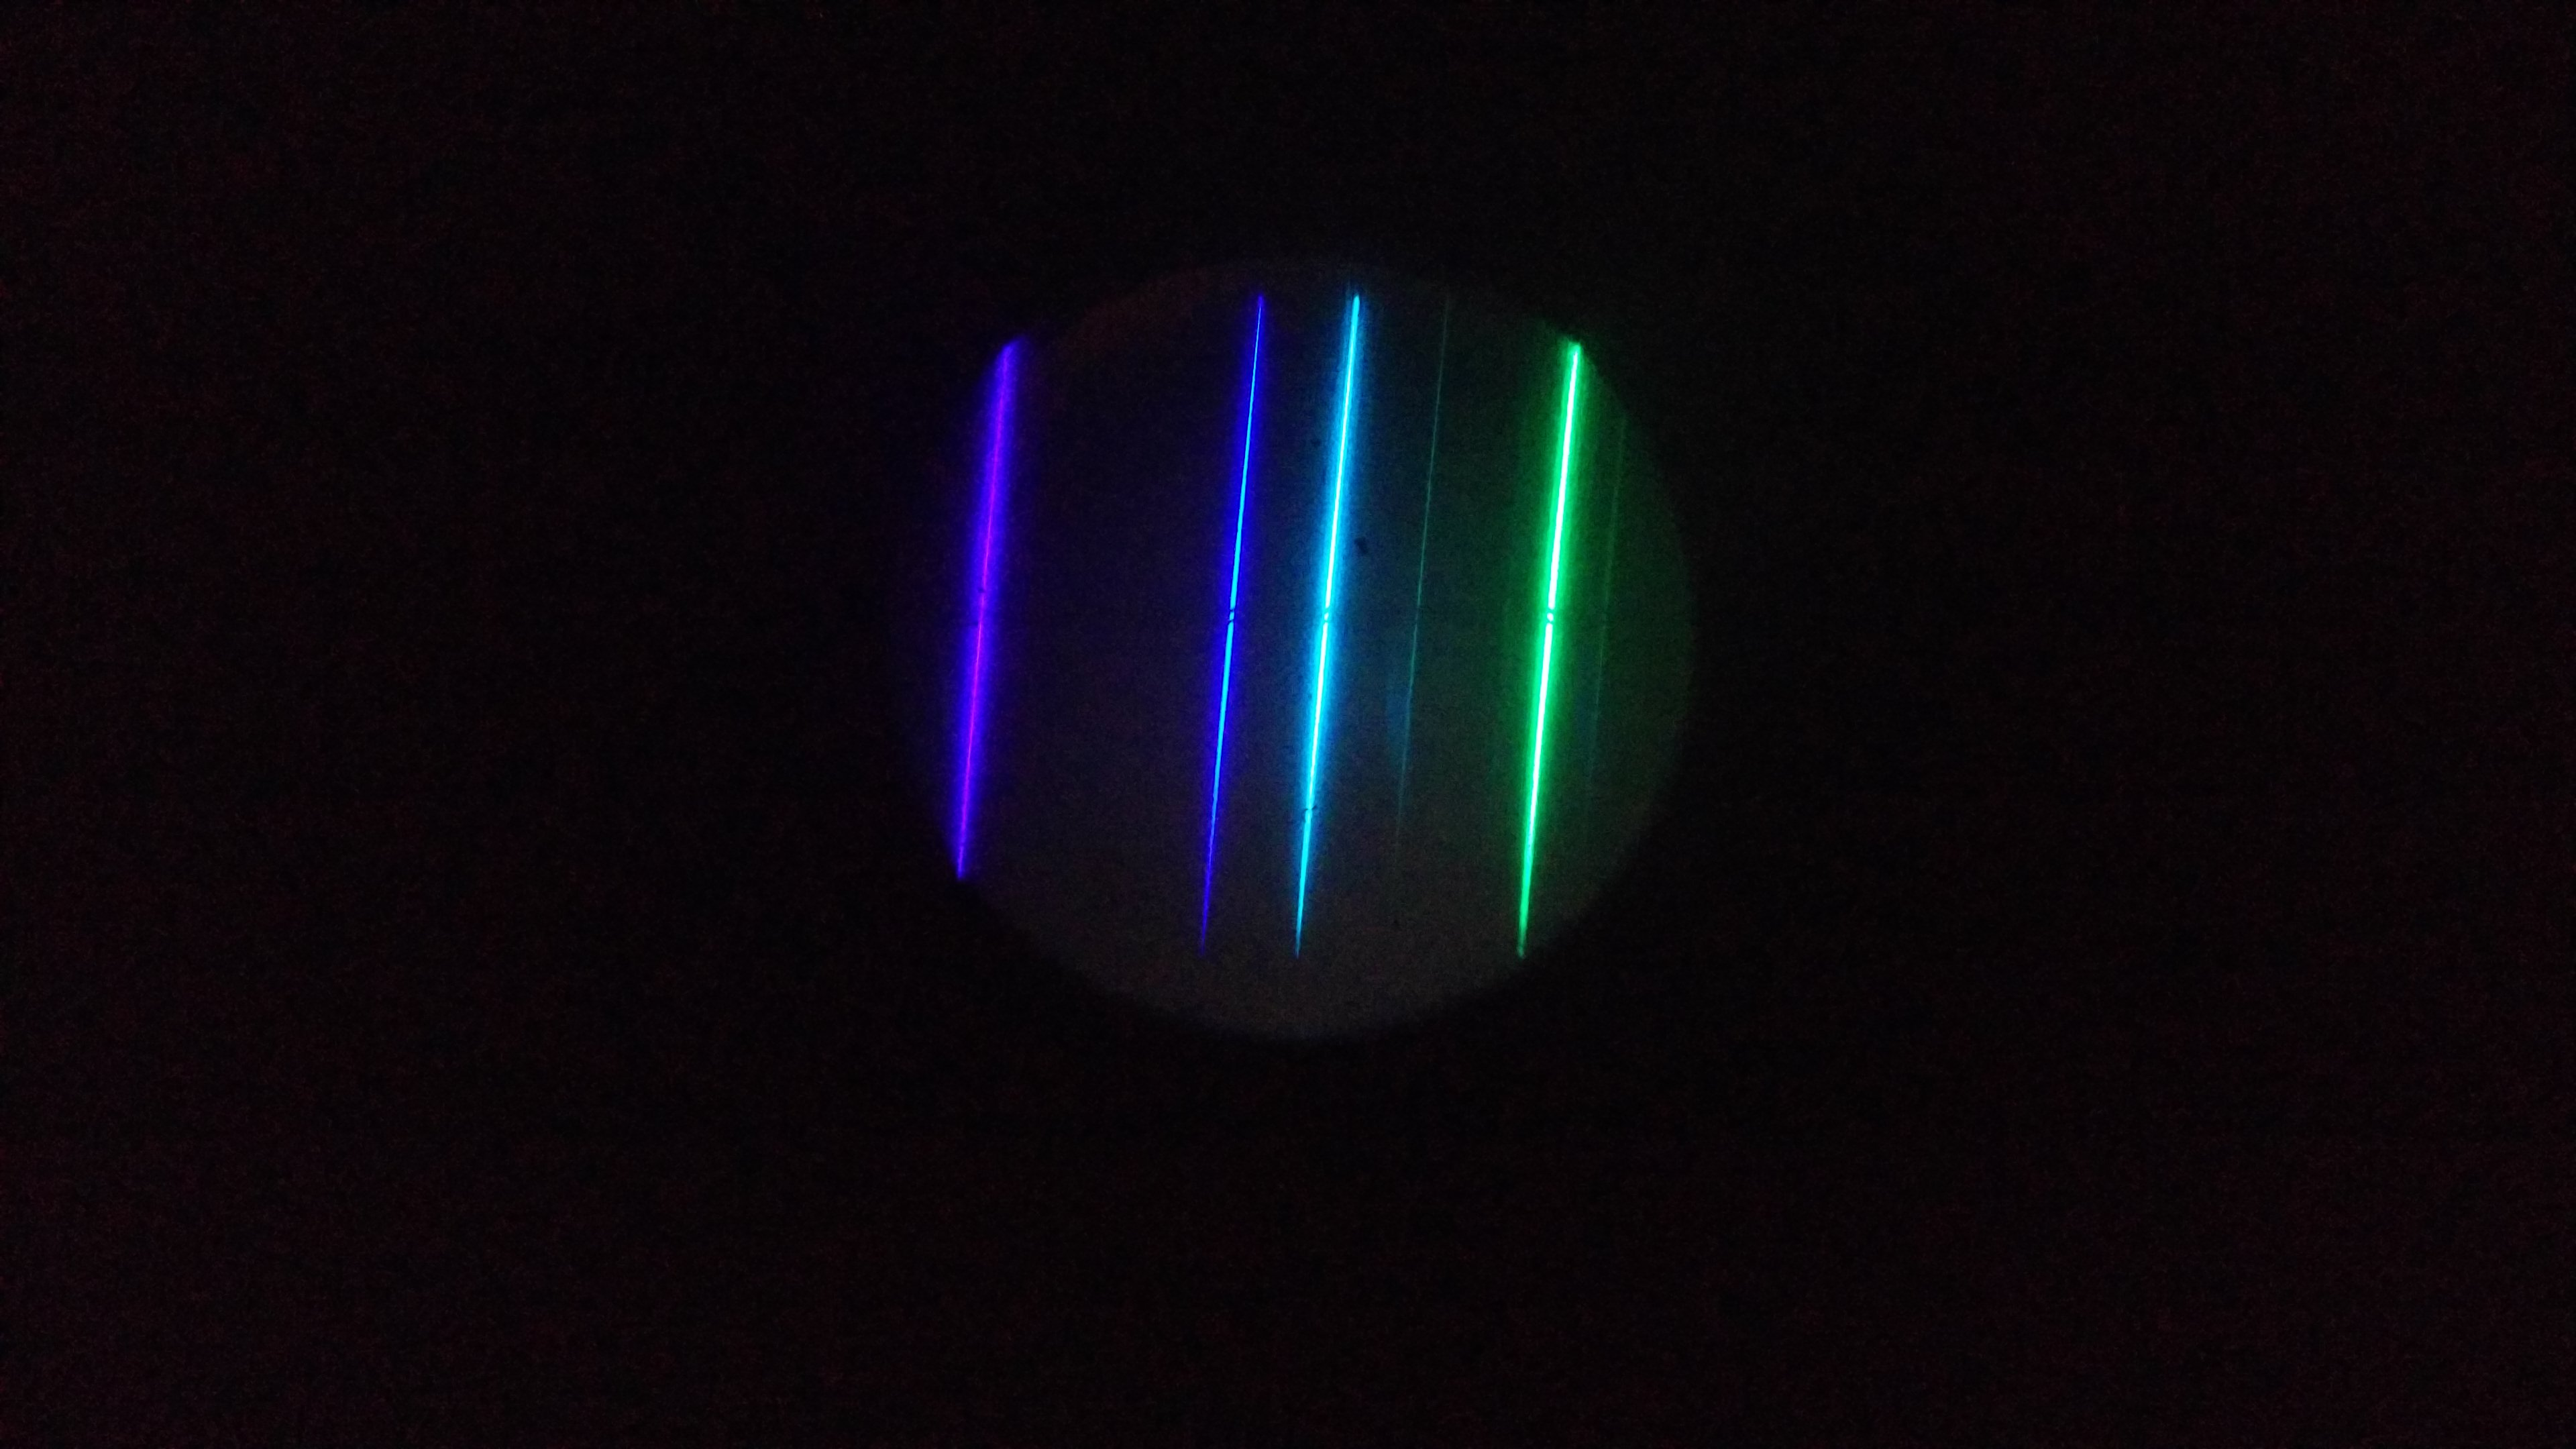
\includegraphics[trim={1cm 1cm 1cm 1cm},clip=true,scale=0.08]{Bilder/IMG_20170915_131047.jpg}  
	\end{center}
	
	\vspace*{\fill}
	\thispagestyle{empty}
\end{titlepage}





\newpage
\thispagestyle{empty}
\tableofcontents
\newpage

%Kopf- und Fußzeile
\pagestyle{fancy}
\fancyhf{}
%Kopfzeile links bzw. innen
\fancyhead[L]{\nouppercase{\leftmark}}
%Kopfzeile rechts bzw. außen
\fancyhead[R]{\thepage}
%Linie oben
\renewcommand{\headrulewidth}{0.5pt}
\fancyfoot[C]{\thepage}


\setcounter{page}{1}

\section{Einleitung}
In dem ersten Teilversuch der Optik werden Spektrallinien von verschiedenen Stoffen durch ein Prisma und ein Beugungsgitter betrachtet und diese beiden Bauelemente charakterisiert.
Dabei wird die Dispersionskurve und das Auflösungsvermögen des Prismas bestimmt, sowie beim Gitter die Gitterkonstante und das Auflösungsvermögen.
Außerdem wird nach erfolgter Charakterisierung mit beiden Bauelementen eine unbekannte Spektrallinie bestimmt.

\section{Prismenspektrometer}
\subsection{Theorie des Prismas}
Ein Lichtbündel, welcher auf eine Grenze von zwei verschiedenen Materialien trifft, wird nach Snellius gebrochen, da jedes Material unterschiedliche Brechungsindizes hat, welche beschreiben wie schnell sich eine Lichtwelle im Medium ausbreitet. Der Brechungsindex ist innerhalb eines Mediums von der Wellenlänge einer Lichtwelle abhängig. Dieses Phänomen heißt Dispersion. 
Die Elektronen im Medium werden durch das E-Feld aus ihrer Ruhelage ausgelenkt und bilden im Dipol-Modell eine zeitlich veränderliche Polarisation. Anders ausgedrückt regt die Lichtwelle die Dipole in einem Medium zum schwingen an. Wenn die Frequenz der Welle und damit die Frequenz der Anregung weit weg von der Eigenfrequenz der Dipole ist, so spricht man von normaler Dispersion. Dabei nimmt die Dispersionskurve $n(\lambda )$ mit steigendem $\lambda $ ab. Im Resonanzfall, also wenn die Frequenz der Lichtwelle nah an der Eigenfrequenz der Dipole liegt, nimmt die Dispersionskurve zu und wir sprechen von annormaler Dispersion. Innerhalb des sichtbaren Spektralbereich tritt allerdings nur normale Dispersion auf.


\begin{figure}[H]
	\centering
	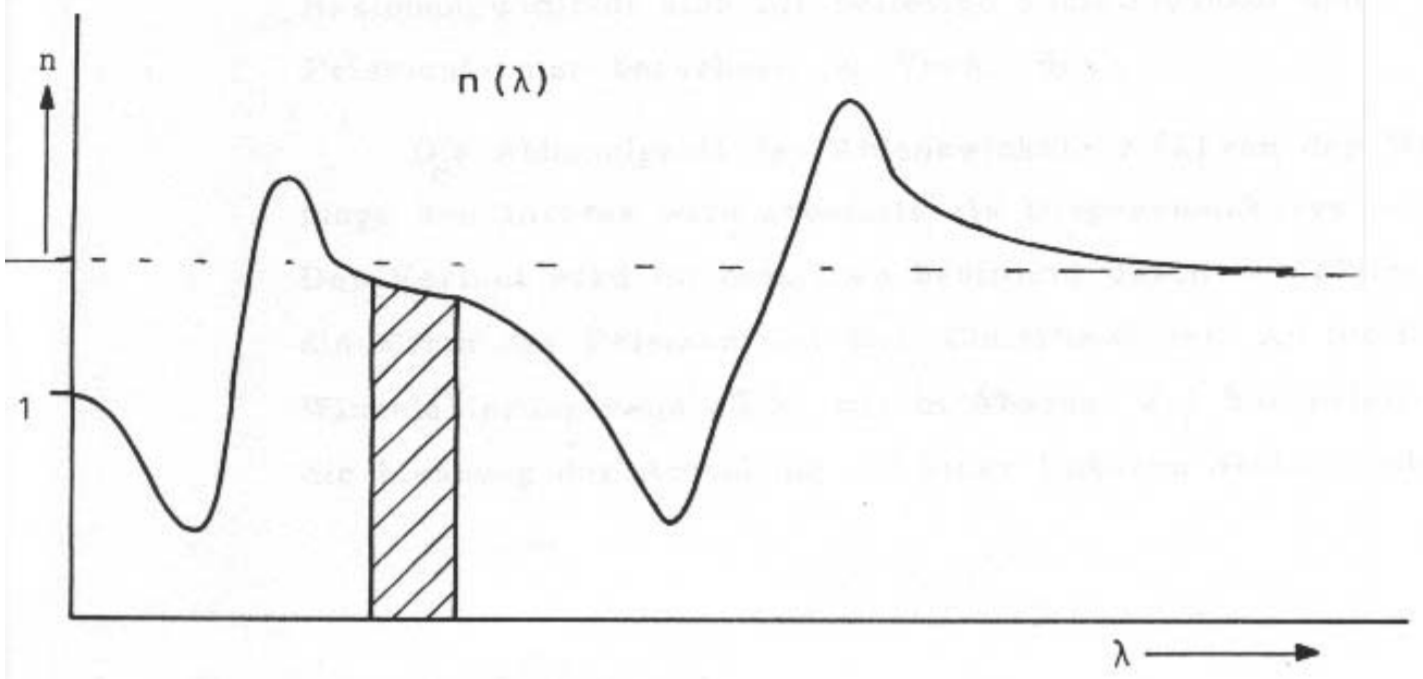
\includegraphics[trim = 0mm 0mm 0mm 0mm,clip, width=9cm]{Bilder/Dispersionskurve.png}%
	\caption[Dispersionskurve]{Dispersionskurve}%
	\label{pic:Abbildung 1}%
\end{figure}



Die Dispersionskurve lässt sich nach der Sellmeier-Formel parametrisieren zu:
\begin{center}
$n^2-1=\frac{a_1}{1-\frac{b_1}{\lambda^2}}+\frac{a_2}{1-\frac{b_2}{\lambda^2}}+a$
\end{center}
Da wir nur die normale Dispersion im sichtbaren Bereich betrachten ergibt eine Taylorentwicklung die folgende Näherung dieser Formel:
\begin{center}
$n(\lambda )=a(1+\frac{b_1}{\lambda^2}+\frac{b_2}{\lambda^4 })$
\end{center}
Das Brechungsgesetz nach Snellius besagt nun, dass sich ein Strahl welcher sich in einem Medium mit Brechungsindex $n_1$ ausbreitet und um einen Winkel $\alpha_1$ auf eine Grenzfläche trifft, (mit $n_2$ als Brechungsindex des zweiten Mediums) so ist der Ausbreitungswinkel zum Lot im zweiten Medium gegeben mit der Formel:
\begin{center}
$n_1 \cdot sin(\alpha_1)= n_2 \cdot sin(\alpha_2)$
\end{center}

Das Prisma ist ein aus Glas bestehender Körper, welcher zwei ebene Begrenzungsflächen besitzt. Diese schließen einen brechenden Winkel $\epsilon$ ein. Ein Lichtstrahl der auf eine Begrenzungsfläche trifft wird nach dem Brechungsgesetz nach Snellius gebrochen.  


\begin{figure}[H]
	\centering
	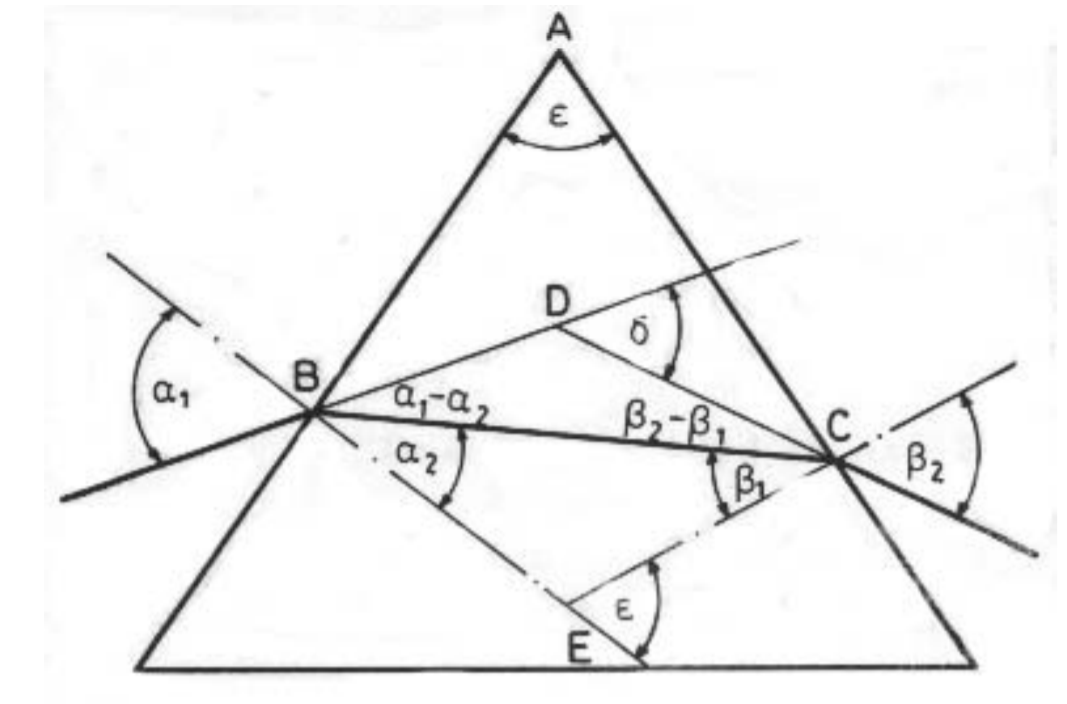
\includegraphics[trim = 0mm 0mm 0mm 0mm,clip, width=9cm]{Bilder/Prismengeometrie.png}%
	\caption[Geometrie eines Prismas]{Geometrie eines Prismas}%
	\label{pic:Abbildung 1}%
\end{figure}



Mit dem Brechungsgesetz, dem Einfallswinkel $\alpha_1$ und dem brechendem Winkel$\epsilon $ kann der Ausfallwinkel $\beta_2$ berechnet werden und damit der Winkel $\delta$, welcher der Winkel zwischen dem einfallendem und ausfallendem Lichtstrahl darstellt.
\begin{center}
$\delta = \alpha_1 -\epsilon +arcsin[\sqrt{n^2-sin^2 (\alpha_1 )} \cdot sin(\epsilon ) -sin(\alpha_1 )\cdot cos(\epsilon )] $
\end{center}

Es kann außerdem ein minimales $\delta$ berechnet werden, welches entsteht, wenn der Strahlengang durch das Prisma symmetrisch ist also $\alpha_1=\beta_2$. In diesem Fall kann man eine Formel für den Brechungsindex des Prisma unabhängig von $\alpha_1$ angeben.
\begin{center}
$n=\frac{sin(\frac{\delta_{min}+\epsilon}{2})}{sin(\frac{\epsilon}{2})}$
\end{center}
Man kann für das Prisma ein Auflösungsvermögen definieren. Wenn man eine bestimmte Wellenlänge $\lambda $ und eine weitere $\lambda + \Delta \lambda$ gerade noch auflösen kann, so ist das Auflösungsvermögen definiert als:
\begin{center}
$A=\frac{\lambda}{\Delta \lambda}$
\end{center}
Beim Prisma kann man das Auflösungsvermögen berechnen mit der Formel $A=\frac{dn}{d\lambda}\cdot S $ wobei diese Formel nur gilt bei gesamter Ausleuchtung des Prismas und S die Seitenlänge ist.
Der erste Faktor bestimmt, wie weit die Linien zusammen liegen, da mit stärkerer Dispersion die Linien stärker zueinander gebrochen werden und die Auflösung besser wird. Der zweite Faktor S beschreibt wie stark Beugungserscheinugen die Auflösung beeinflussen, wenn wir S als Einzelspaltgröße annehmen. Bei kleinerem S, wird der Spalt kleiner und die Beugung stärker. Dadurch werden die Linien breiter und die Auflösung schlechter.
Sollte das Prisma nicht ganz ausgeleuchtet sein sondern nur einen Teil a der Seitenlänge gilt:
\begin{center}
$A=\frac{dn}{d\lambda}\cdot 2a \cdot \frac{sin(\frac{\epsilon}{2})}{cos(\frac{\delta_{min}+\epsilon}{2})}$ 
\end{center}

\subsection{Versuchsaufbau}\label{Aufbau}

\begin{figure}[H]
	\centering
	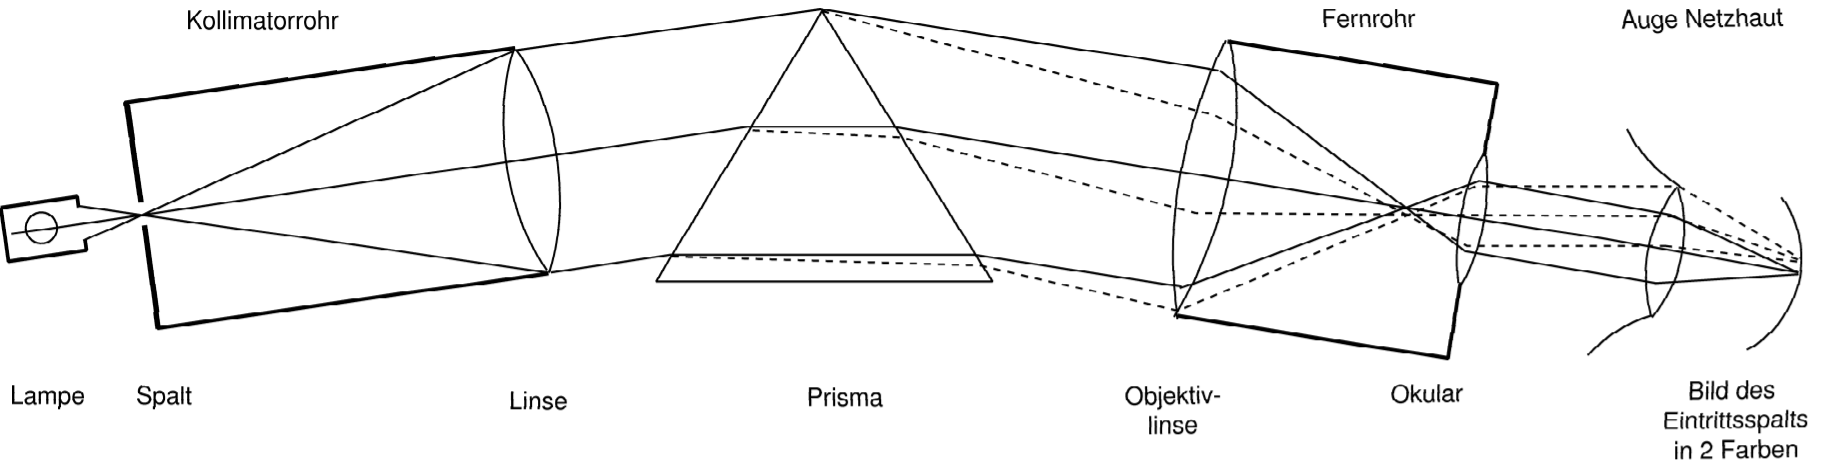
\includegraphics[trim = 0mm 0mm 0mm 0mm,clip, width=12cm]{Bilder/Aufbaugezeichnet.png}%
	\caption[Strahlengang im Aufbau]{Strahlengang im Aufbau}%
	\label{pic:Abbildung 1}%
\end{figure}


Das Licht einer Spektrallampe wird durch ein Prismenspektrometer beobachtet, welches zunächst aus einem Spalt besteht um eine punktförmige Lichtquelle zu simulieren. Dieser Spalt befindet sich in einem Kollimatorrohr und im Brennpunkt einer Sammellinse, die aus den radialen Strahlen des Spaltes eine ebene Lichtwelle macht. Diese ebene Welle wird dann auf ein Prisma geschickt und dann in ein Fernrohr, welches aus einem Objektiv mit großer Brennweite und einem Okular mit kleiner Brennweite besteht, wobei die beiden Brennweiten der Linsen im selben Punkt zusammen fallen. In dem Fernrohr ist noch ein Fadenkreuz eingebaut.
Die nun wieder parallelen strahlen werden dann mit dem Auge beobachtet und das Bild entsteht dann auf der Netzhaut des Auges.
Da die verschiedenen Spektrallinien des Lichtes unterschiedliche stark im Prisma gebrochen werden, kann man das Bild des Spalten unter verschiedenen Winkeln mehrmals in den verschiedenen Farben der Spektrallinien sehen.
Auf der Apparatur kann man den Winkel zwischen Fernrohr und Kollimatorrohr anhand einer Winkelskala mit Nonius ablesen. Außerdem kann man den Teller auf dem sich das Prisma befindet ebenfalls drehen.
An der Apparatur kann man mehrere Schrauben einstellen um Drehteller des Prismas mit dem Drehteller des Fernrohrs parallel zu stellen.
Dazu wird eine Dosenlibelle zur Hilfe genommen.
Außerdem kann man die Höhe des Fernrohrs und des Kollimatorrohres einzeln einstellen, sowie die Höhe des Spalts.

\begin{figure}[H]
	\centering
	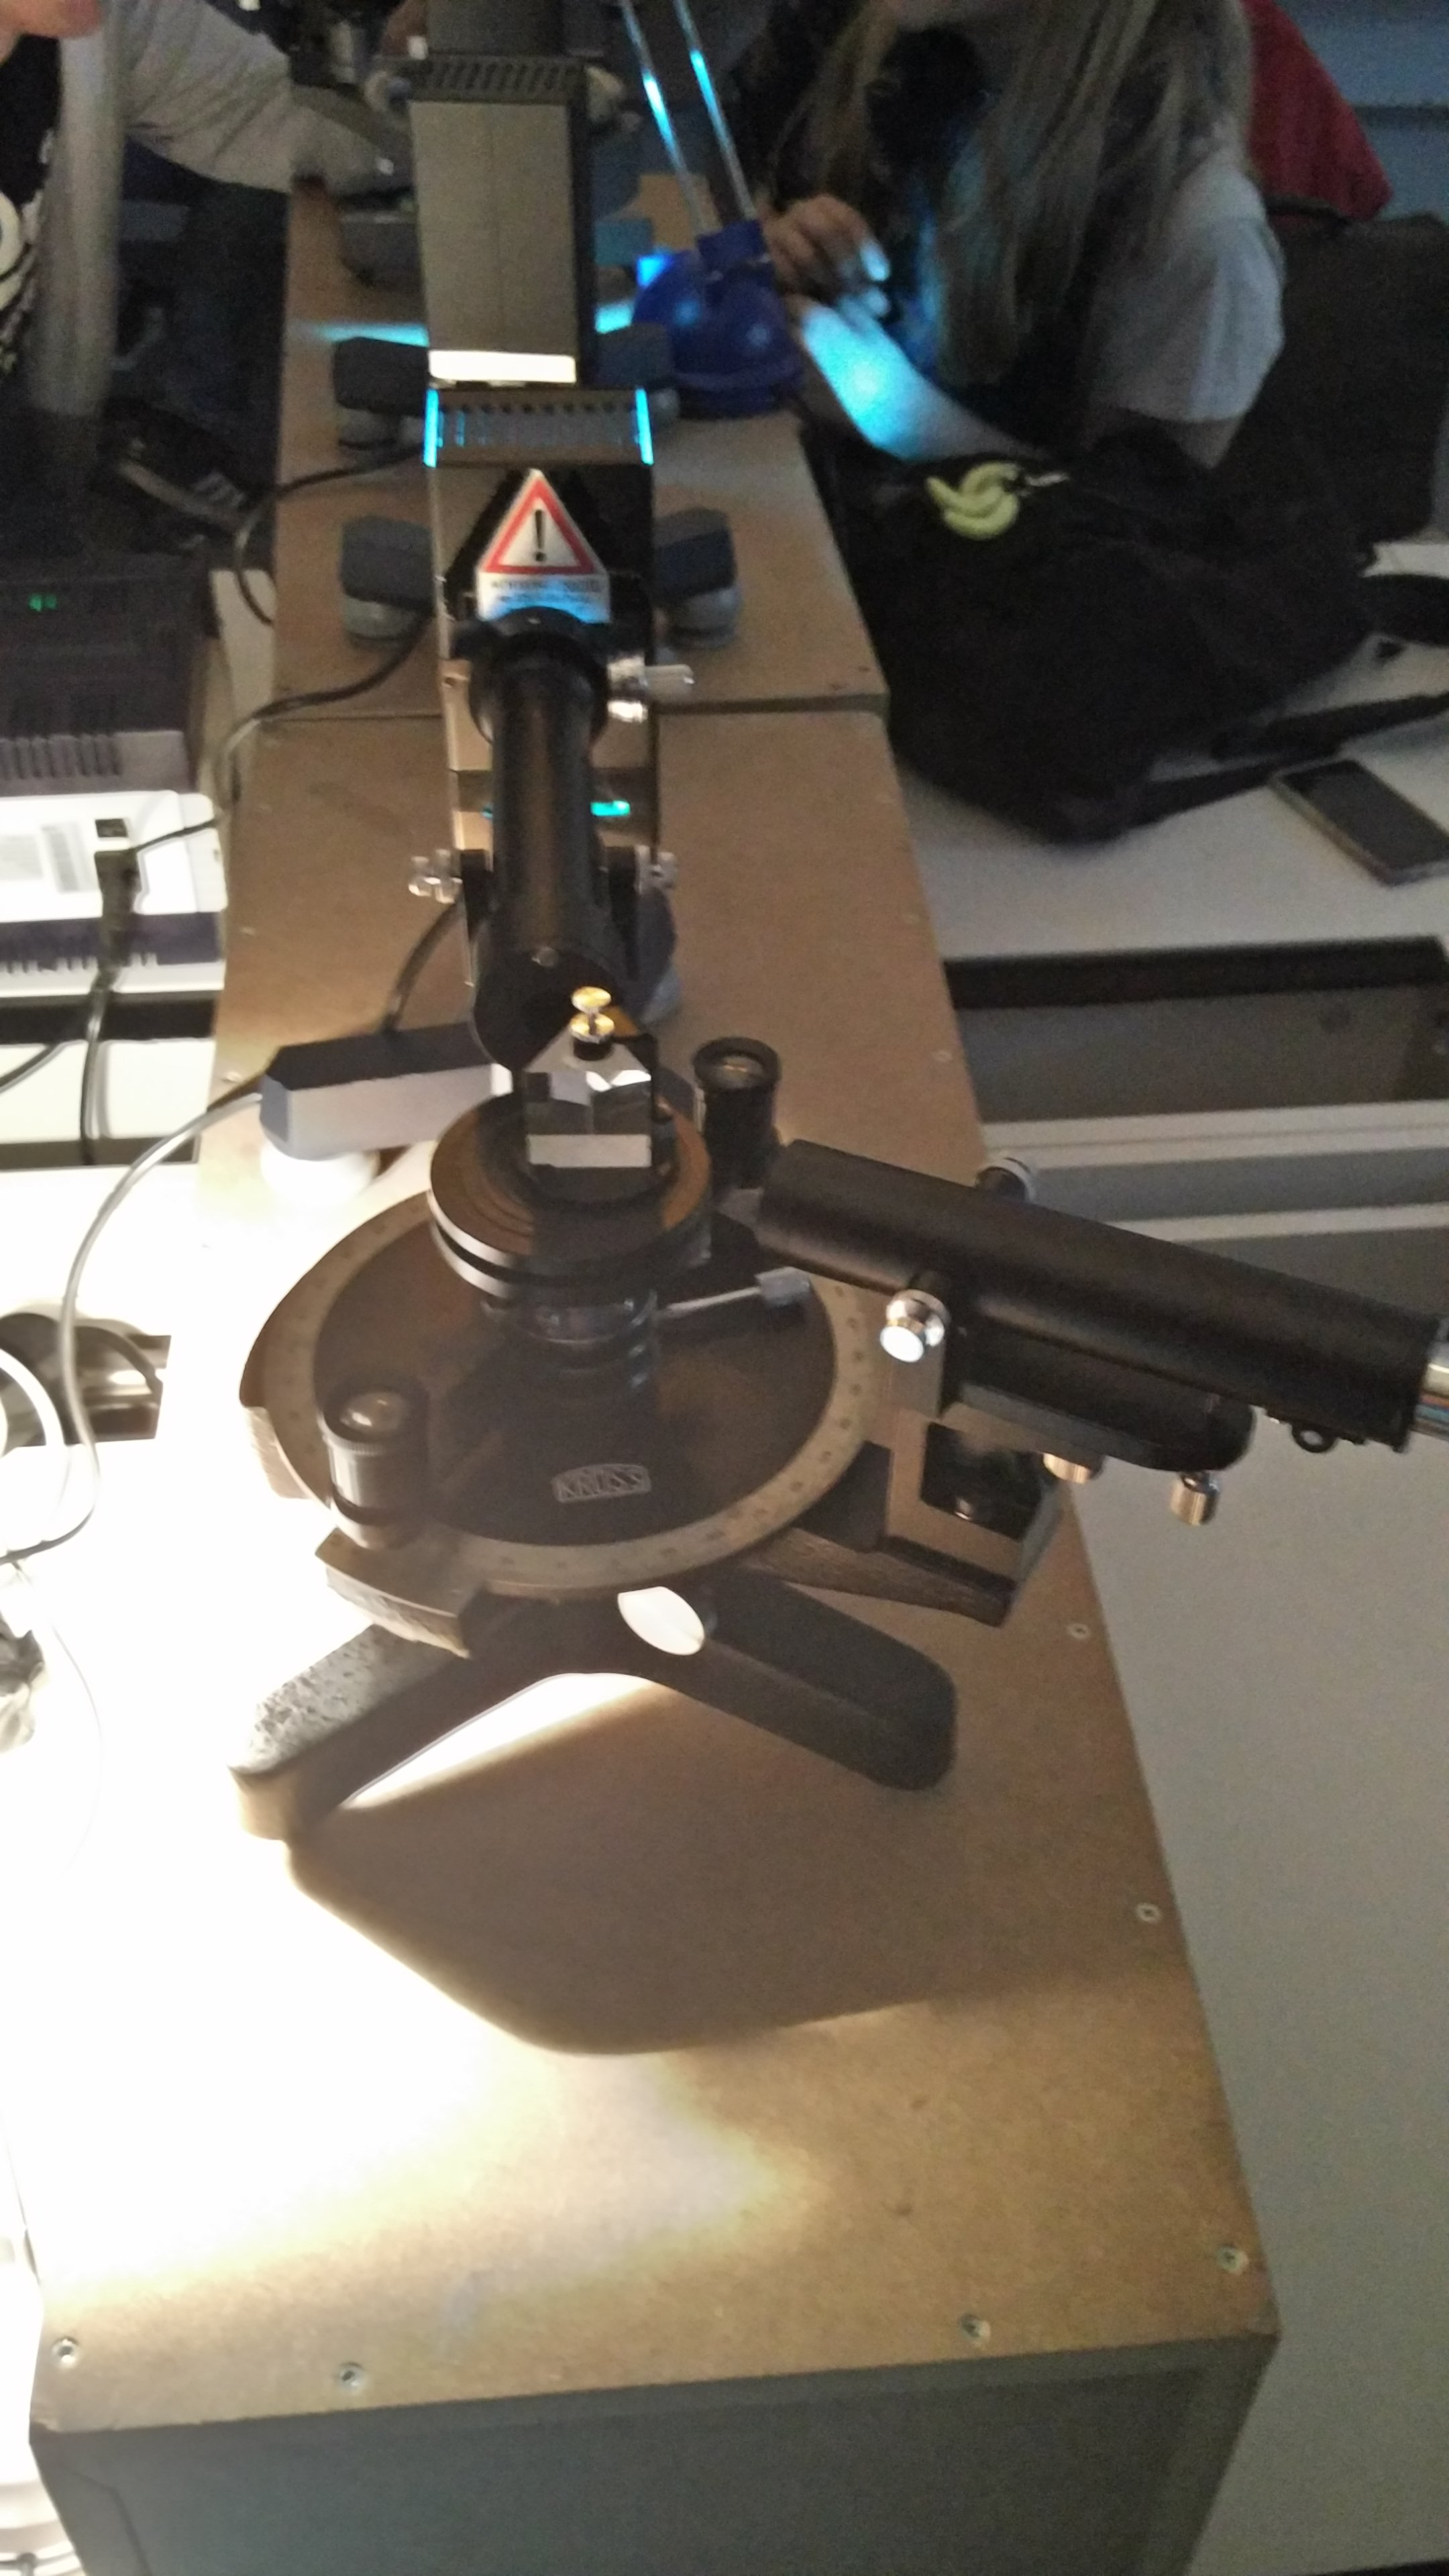
\includegraphics[trim = 0mm 15cm 0mm 20cm,clip, width=7cm]{Bilder/IMG_20170915_131253.jpg}%
	\caption[Aufbau mit Prisma]{Aufbau mit Prisma}%
	\label{pic:Abbildung 1}%
\end{figure}


\subsection{Durchführung}
Zunächst wird eine HgCd Lampe als Lichtquelle benutzt und das Prisma so auf den Teller gelegt, dass die gebrochenen Linien auf einer Seite zu sehen sind. Für jede Linie wird nun der minimale Ablenkungswinkel $\delta_{min}$ eingestellt, indem Prismenteller solange gedreht wird, bis sich die Linie des Spalts nicht mehr mitdreht und in die andere Richtung wandert. Das Fadenkreuz im Fernrohr wird nun auf die Linie gerichtet und der Winkel auf der Noniusskala wird abgelesen und notiert. Dieser Vorgang wird 3 mal pro ausgewählte Linie wiederholt. Dannach wird das Prisma auf dem Prismenteller so gedreht, dass die gebrochenen auf der anderen Seite der Apparatur beobachtet werden. Der gesamte Vorgang wird wiederholt und ebenfalls alle Winkeleinstellungen pro Spektrallinien drei mal aufgeschrieben. Bei einer Spektrallinie und einer Seite wird der Vorgang 10 mal wiederholt, da daraus später der Fehler auf einen Mittelwert einer Winkeleinstellung bestimmt wird.\newline
Nun wird die gesamte Messung mit einer Zn Lampe für alle Linien wiederholt. 
Zum Schluss wird wieder die HgCd Lampe werwendet und vor dem Prisma eine in der Breite verstellbare Blende eingebaut. Im Fernrohr wird nur die gelbe Doppellinie von Quecksilber betrachtet und die Blende immer weiter verringert. Wenn die beiden gelben Linien nicht mehr nebeneinander scharf unterscheidbar sind, wird die Breite der eingestellten Blende notiert und später zur Auswertung des Auflösungsvermögen benutzt.

\subsection{Auswertung}
Zunächst wird mit den Werten der HgCd Lampe die Dispersionskurve des Prismas bestimmt.
Dabei wurden die Winkeleinstellungen folgender Linien benutzt und der Mittelwert bestimmt.
\begin{center}

\begin{tabular}{|c|c|c|c|}
\hline Farbe & Wellenlänge in $nm$ & Winkel der linken Messung& Winkel der rechten Messung \\
\hline dunkel-violett& $404.66$ &$155.033 $&$24.533 $\\
\hline violett &   $435.83$ &$153.339 $&$ 26.228$\\
\hline blau &       $467.81$ &$152.083 $&$ 27.522$\\
\hline blau&   $479.99$ &$151.650 $&$27.872 $\\
\hline blau-grün & $546.07$ &$150.867 $&$28.728 $\\
\hline grün &  $546.07$ &$150.050 $&$29.478 $\\
\hline gelb &   $576.96$ &$ 149.544$&$ 30.017$\\
\hline rot & $643.85$ &$148.644 $&$30.853 $\\
\hline 
\end{tabular}
\end{center}

Die rote Linie der rechten Seite wurde 10 mal gemessen und daraus der Fehler auf eine Messung bestimmt.
\begin{center}
$\sigma_{\psi}=0.016$
\end{center}
Der minimale Auslenkungswinkel $\delta_{min}$ kann berechnet werden durch die Formel: $\delta_{min}=\frac{\psi_2-\psi_1}{2}$.
Dadurch kann mit der folgenden Formel für jede Wellenlänge ein Brechungsindex des Prismas berechnet werden.
\begin{center}
$n=\frac{sin(\frac{\delta_{min}+\epsilon}{2})}{sin(\frac{\epsilon}{2})}\;\;\;\;\;\;\; \sigma_n=\frac{cos(\frac{\epsilon+\delta}{2})\cdot \sigma_{\delta}}{2\cdot sin(\frac{\epsilon}{2})}$
\end{center}

\begin{center}
\begin{tabular}{|c|c|c|}
\hline Farbe & $\delta_{min}$ & n\\
\hline dunkel-violett &$65.250$&$1.77603 \pm 0.00006$\\
\hline violett &$63.556$&$1.76224 \pm0.00006 $\\
\hline blau  &$62.281$&$1.75161 \pm0.00006 $\\
\hline blau&$61.889$&$1.74830 \pm0.00006 $\\
\hline blau-grün  &$61.070$&$ 1.74131\pm0.00006 $\\
\hline grün &$60.286$&$1.73454 \pm0.00006 $\\
\hline gelb &$ 59.764$&$1.72999 \pm0.00006 $\\
\hline rot &$58.896$&$1.72233 \pm 0.00005$\\
\hline 
\end{tabular}
\end{center}
Der Fehler auf $\delta_{min}$ berechnet sich zu $\sigma_{\delta_{min}}=\frac{\sigma_{\psi}}{\sqrt{6}}=0.007$ . Außer bei der roten Linie zu$\sigma_{\delta_{min}}=\frac{\sqrt{13}\cdot \sigma_{\psi}}{\sqrt{90}}=0.006$.

Nun werden die Brechungsindizes n über $\frac{1}{\lambda^2}$ aufgetragen und mit Python ein Fit durchgeführt welcher die Parameter $a,b_1$ und $b_2$ in der getaylorten Sellmeier-Formel anpasst.
\begin{center}
$n(\lambda )=a(1+\frac{b_1}{\lambda^2}+\frac{b_2}{\lambda^4 })$
\end{center}


\begin{figure}[H]
	\centering
	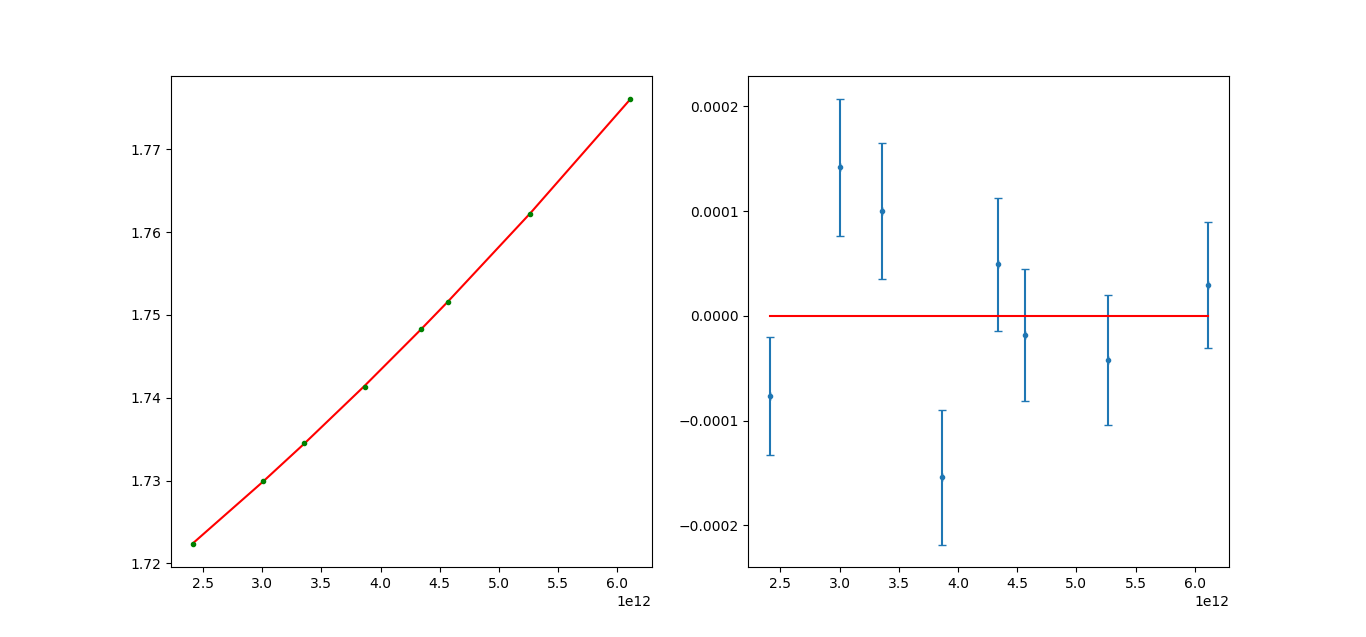
\includegraphics[trim = 0mm 0mm 0mm 0mm,clip, width=15cm]{Bilder/nicht_linearer_fit.png}%
	\caption[nicht linearer Fit]{nicht linearer Fit}%
	\label{pic:Abbildung 1}%
\end{figure}

\begin{center}
\begin{tabular}{|c|c|c|c|}
\hline a & $b_1$ & $b_2$ & $\frac{\chi^2}{ndof}$  \\
\hline  $1.6966\pm 0.0003 $&$(5.41 \pm 0.08)\cdot 10^{-15} m^2 $&$(3.7 \pm 0.1)\cdot 10^{-28}m^4 $& $4.09 $\\
\hline
\end{tabular}
\end{center}

Außerdem wird einmal $b_2$ gleich null gesetzt und eine einfache lineare Regression durch zu führen.
\begin{center}
$n(\lambda)=\frac{a}{\lambda^2}+b$
\end{center}
\begin{figure}[H]
	\centering
	\hskip -2cm
	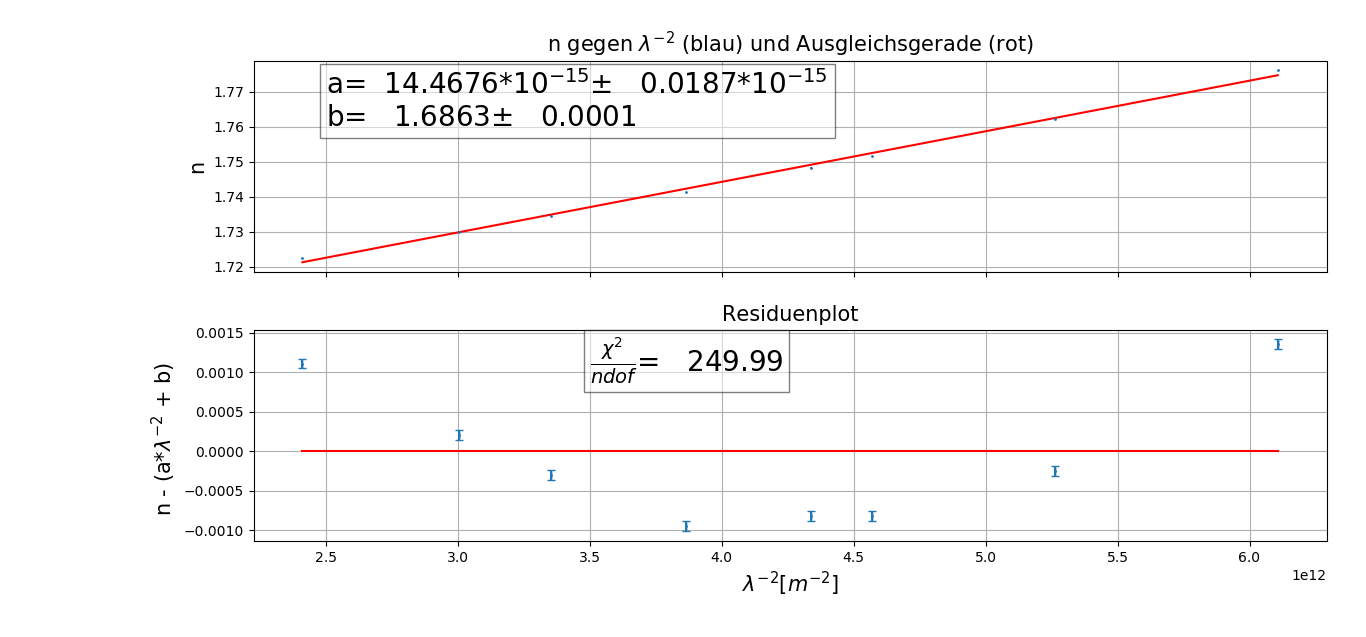
\includegraphics[trim = 0mm 0mm 0mm 0mm,clip,scale=0.5]{Bilder/lineare_fit.png}%
	\caption[lineare Regression]{lineare Regression}%
	\label{pic:Abbildung 1}%
\end{figure}
 
 \begin{center}
\begin{tabular}{|c|c|c|}
\hline a & b & $\frac{\chi^2}{ndof}$  \\
\hline  $(1.445 \pm 0.0017)\cdot 10^{-14}m^2 $&$1.6864 \pm 0.0001 $&$323 $\\
\hline
\end{tabular}
\end{center}

Nun werden die Wellenlängen der Zn Lampe durch die bekannte Dispersionskurve und die abgelesenen Winkel bestimmt.
Dadurch werden zunächst einmal wieder $\delta_{min}$ und damit n wie oben bestimmt.
\begin{center}
\begin{tabular}{|c|c|c|c|c|c|}
\hline Farbe & $\lambda_{theo}$ in $nm$ & linke Messung& rechte Messung& $\delta_{min}$ & n \\

\hline blau&$468.01$ &$152.011 $&$27.523 $&$62.245 $&$1.75131 \pm 0.00006$\\
\hline blau&$472.22$ &$151.861 $&$27.661 $&$62.100 $&$1.75009 \pm 0.00006$\\
\hline blau&$481.05$ &$151.567 $&$27.928 $&$61.820 $&$1.74771 \pm 0.00006$\\
\hline rot &$636.23$ &$148.707 $&$30.811 $&$58.948 $&$1.74228 \pm 0.00006$\\
\hline 
\end{tabular}
\end{center}



Durch invertieren der Dispersionskurve erhält man:
\begin{center}
$\lambda^2=\frac{a\cdot b_1 \pm \sqrt{a^2 \cdot b_1^2+4a\cdot b_2(n-a)}}{2(n-a)}$
\end{center}
Wobei hier immer die positive Lösung benutzt wird.
Damit berechnen sich die berechneten Wellenlängen zu.

\begin{center}
\begin{tabular}{|c|c|c|c|c|c|}
\hline Farbe & $\lambda_{theo}$ in $nm$ & $\lambda_{exp}$ in $nm$& Abweichung in $\sigma$\\

\hline blau&$468.01$ &$468.91 \pm 0.20 $&$4.71 $\\
\hline blau&$472.22$ &$473.21 \pm 0.21$&$4.99 $\\
\hline blau&$481.05$ &$482.04\pm 0.22 $&$4.61 $\\
\hline rot &$636.23$ &$639.94\pm 0.63 $&$5.43 $\\
\hline 
\end{tabular}
\end{center}
In der Formel für den Fehler auf $\lambda$ ist $b_1=b$ und $b_2=c$.
\begin{center}
$\sigma_{\lambda} = \frac{a (b \sqrt{a (a b^2 - 4 a c + 4 c n)} + a (b^2 - 2 c) + 2 c n)}{2 \sqrt{2} (a - n)^2 \sqrt{a (a (b^2 - 4 c) + 4 c n)} \sqrt{-\frac{\sqrt{ a (a b^2 - 4 a c + 4 c n))} + a b}{a - n}}}\cdot \sigma_n$
\end{center}


Das Auflösungsvermögen des Prismas wird durch die Formel bestimmt
\begin{center}
$A_{exp}=\frac{dn}{d\lambda}\cdot 2a \cdot \frac{sin(\frac{\epsilon}{2})}{cos(\frac{\delta_{min}+\epsilon}{2})}$ 
\end{center}
Beim Betrachten der gelben Doppellinie der HgCd Lampe ($\lambda=579.07nm$ $\Delta \lambda=2.11nm$) wurde die Blende und damit die Beleuchtungsfläche a soweit verkleinert, bis die Doppellinie nicht mehr auflösbar war.
Bei einer Spaltbreite von $a=1mm$ konnte man die beide Linien gerade noch durch einen Schatten in der Mitte einer gelben Linie auflösen.
Damit ergibt sich ein berechnetes Auflösungsvermögen von
\begin{center}
$A_{exp}=268.8$
\end{center}
Das mindestens benötigte Auflösungsvermögen der Doppellinie kann als untere Grenze dienen und beträgt: $A_{theo}=\frac{\lambda}{\Delta \lambda}=274.44$

\subsection{Fazit zu den Versuchen zum Prisma}
Bei den beiden Fits ist auffällig, dass obwohl der Koeffizient $b_2$ im nicht linearen Fit verschwindend klein ist, es trotzdem von Vorteil ist ihn zu betrachten, da das $\frac{\chi^2}{ndof}$ im nicht linearen Fit sehr viel besser ist, als im linearen Fit. Wir vermuten, dass dies aus den kleinen Fehlern von den Brechungskoeffizienten n herrührt und dadurch selbst eine kleine Systematik sofort im Residuenplot auffällt.
Mit der vorher bestimmten Dispersionskurve konnten die Wellenlängen der Spektrallinien von Zink zwar nur unter mehreren Standartabweichungen genau bestimmt werden, allerdings kann trotzdem die Sellmeier-Formel mit diesen Ergebnissen bestätigt werden.
Das berechnete Auflösungsvermögen ist etwas unterhalb des benötigten Auflösungsvermögen der gelben Doppellinie von Hg. Allerdings ist dieser Wert sehr Fehler abhängig und vor allem seine Messung objektiv. Trotzdem konnten wir die ungefähre Größenordnung treffen.


\clearpage
\section{Gitterspektrometer}

\subsection{Theoretische Grundlagen der Gitterspektroskopie}

\begin{figure}[H]
	\centering
	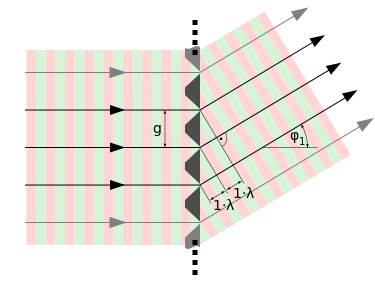
\includegraphics[scale=0.8]{./Bilder/Beugungsgitter-erstes-Maximum.png}
	\caption{Interferenz von ebenen Wellen am Gitter, mit Gangunterschied $\Delta=\lambda$ für das Maximum erster Ordnung \protect \footnotemark}
	\label{pic:Gitter}	
\end{figure}
\footnotetext{Quelle:Wikipedia - \url{https://commons.wikimedia.org/wiki/File:Beugungsgitter-erstes-Maximum.svg}}

Ein Gitter wird charakterisiert durch die Spaltbreite $b$, Gitterkonstante $d$ und die Anzahl der \textbf{ausgeleuchteten} Spalte $N$. Auf das Gitter treffen parallele, ebene Wellenfronten (\textit{Fraunhofer-Beugung}) und werden an den Spalten gebeugt, wobei jeder Punkt der Spaltöffnungen Ausgangspunkt einer gleichphasigen Kugelwelle ist (\textit{Huygenssches Prinzip}).

Für den Gangunterschied  der Teilwellen, die konstruktiv miteinander interferieren, lässt sich folgender Zusammenhang aufstellen:
\begin{equation}\label{eq:IGitter}
\Delta = g \cdot \sin(\varphi_n) = n \cdot \lambda
\end{equation}
In Abbildung \ref{pic:Gitter} ist dies für das Maximum erster Ordnung gezeigt.

Falls das Gitter jedoch nicht senkrecht zum Strahlengang ausgerichtet ist, muss zusätzlich der Gangunterschied \textbf{vor} dem Gitter berücksichtigt werden:
\begin{equation}\label{eq:GitterVerdreht}
n \cdot \lambda = g \cdot (\sin(\vartheta)+\sin(\phi_n-\vartheta))
\end{equation}
Hier ist jetzt $\phi_n$ der Winkel zwischen Einfallsstrahl und Beobachtungsrichtung und $\vartheta$ der Drehwinkel des Gitters zum Lot hin.

Es ergibt sich, dass die Lage der Intensitätsmaxima antiproportional zu Wellenlänge des Lichts ist. Der Beugungswinkel (also Linienabstand) ist antiproportional zum Spaltabstand.
Die Hauptmaxima des Gitters werden mit wachsender Spaltanzahl schmaler und steiler. Außerdem befinden sich zwischen diesen noch $N-2$ Nebenmaxima, deren Intensität jedoch mit $N^2$ abnimmt, wodurch diese im Versuch garnicht sichtbar sind.


\clearpage
\paragraph{Auflösungsvermögen}
Das spektrale Auflösungsvermögen des Gitters lässt sich mit Hilfe des \textit{Rayleigh-Kriteriums} herleiten und beträgt
\begin{equation}\label{eq:AGitter}
A = \frac{\lambda}{\Delta\lambda} = n \cdot N
\end{equation}
Dabei nimmt man an, dass wir Spektrallinien genau dann noch trennen können, wenn das Maximum der ersten Linie im Minimum der zweiten liegt.




\subsection{Aufbau}
Der Aufbau des Gitterspektrometers ist analog zu dem vom Prismenspektrometer (siehe \ref{Aufbau}), nur das jetzt ein Gitter in den Strahlengang gestellt wird. Dabei muss darauf geachtet werden, dass dieses senkrecht zum einfallenden Strahl steht, da sonst bereits vor dem Gitter ein Gangunterschied der Strahlen vorliegt und die Lage der Maxima sich dadurch verschiebt. Da dies mit den zur Verfügung stehenden Mitteln aber nicht sichergestellt werden kann, muss später bei der Auswertung untersucht werden, ob das Gitter schräg stand.

Außerdem wird bei diesem Versuch zusätzlich zur \texttt{HgCd}-Lampe eine \texttt{Na}-Lampe verwenden, um die Wellenlänge der Natrium-Doppellinie und Anhand dieser das Auflösungsvermögen des Gitters zu bestimmen.


\subsection{Durchführung}
Das grundlegende Vorgehen ist ähnlich zu dem beim Prismenspektrometer: durch Ausrichtung des Fernrohrs auf die einzelnen Spektrallinien und Ablesen des Nonius werden die Beugungswinkel vermessen.

Der gesamte Versuch wurde mit einem Gitter mit 600 Strichen$/mm$ durchgeführt.

Zu Beginn wird die Nulllinie (Maximum 0.-Ordnung) der \texttt{HgCd}-Lampe durch 10-fache Messung bestimmt. Es wird angenommen, dass der statistische Fehler auf die folgenden Messungen gleich bleibt, daher werden die Linien im folgenden nurnoch 3 Mal ausgemessen.

\subsubsection{Bestimmung der Gitterkonstante}
Zunächst werden die Wellenlängen der Spektrallinien der \texttt{HgCd}-Lampe als bekannt angenommen (diese stammen aus der \texttt{NIST}-Datenbank und haben nur sehr geringe Unsicherheiten, und werden daher als nicht fehlerbehaftet angenommen) und die Beugungswinkel $\phi_n$ werden gemessen. Dabei konnte nur bis zur zweiten Ordnung beobachtet werden. Leider konnten aus Zeitgründen nur 4 Spektrallinien (die am besten sichtbarsten) vermessen, die in Tabelle \ref{table:SpektrumHgCd} dargestellt sind. Die Winkel wurden immer 3 Mal gemessen und gemittelt, jeweils bis zur zweiten Ordnung auf beiden Seiten.

\begin{table}[H]
	\large
	\centering
	\begin{tabular}{|c|c|c|}
		\hline
		Element & Wellenlänge $[nm]$ & Farbe \\
		\hline
		Cd & 467.81 & blau \\
		\hline
		Cd & 508.58 & grün \\
		\hline
		Hg & 576.96 & gelb \\
		\hline
		Cd & 643.85 & rot \\
		\hline
	\end{tabular}
	\caption{Zur Vermessung ausgewählte Spektrallinien der \texttt{HgCd}-Lampe (Werte stammen aus der \texttt{NIST}-Datenbank)}
	\label{table:SpektrumHgCd}
\end{table}

Der Beugungswinkel ist dabei immer die Differenz des gemessenen Winkels und der Nulllinie. Aus den Winkel kann dann durch eine lineare Regression die Gitterkonstante bestimmt werden.

\subsubsection{Bestimmung der Wellenlängen der \texttt{Na}-Doppellinie}
Mit Hilfe der Zuvor bestimmten Gitterkonstante wird nun die Natrium-Doppellinie ausgemessen. Auch hier wurde bis zur zweiten Ordnung auf beiden Seiten 3 Mal gemessen und gemittelt.


Die ermittelten Werte werden mit den realen Werte in Tabelle \ref{table:SpektrumNa} verglichen.

\begin{table}[H]
	\large
	\centering
	\begin{tabular}{|c|c|}
		\hline
		Wellenlänge $[nm]$ & Farbe \\
		\hline
		589.59 & gelb \\
		\hline
		589.00 & gelb \\
		\hline
	\end{tabular}
	\caption{\texttt{Na}-Doppellinie (Werte stammen aus der \texttt{NIST}-Datenbank)}
	\label{table:SpektrumNa}
\end{table}

\subsubsection{Bestimmung des Auflösungsvermögens}
Das Auflösungsvermögen des Gitters wird auch anhand der \texttt{Na}-Doppellinie bestimmt (dieses ist unabhängig von Wellenlänge oder Gitterkonstante (!) wie in Gleichung \ref{eq:AGitter} zu sehen).
Um die Abhängigkeit von der Anzahl $N$ der ausgeleuchteten Spalte zu realisieren, wird eine Schlitzblende verwendet, die feste Schlitzbreiten von $0,5mm$ bis $6mm$ in $0,5mm$-Schritten bietet. Es wird beobachtet, bei welcher Schlitzbreite die Doppellinie nicht mehr unterscheidbar wird. Dieses Ergebnis wird dann mit dem nach der Formel minimal benötigten Auflösungsvermögen ($A=589nm/0.59nm\approx998.3$) verglichen.



\clearpage
\subsection{Auswertung}
\subsubsection{Bestimmung der Beugungswinkel}\label{Bestimmung der Beugungswinkel}
Da die abgelesenen Winkel nicht den Winkeln bezüglich der Lichteinfallsrichtung entsprechen, müssen diese zunächst umgerechnet werden, indem man den Nullwinkel $\varphi_0$ (Tabelle \ref{table:Nulllinie}) von diesen abzieht:
\begin{equation}
\varphi_n = \varphi_{n, gemessen} - \varphi_0
\end{equation}

\begin{table}[H]
	\large
	\centering
	\begin{tabular}{|c|c|}
		\hline
		Messung &	abgelesener Winkel \\
		\hline
		1	&	$206.5^{\circ} \, 0'$ \\
		\hline
		2	&	$206.0^{\circ} \, 25'$ \\
		\hline
		3	&	$206.5^{\circ} \, 0'$ \\
		\hline		
		4	&	$206.0^{\circ} \, 29'$ \\
		\hline
		5	&	$206.5^{\circ} \, 1'$ \\
		\hline
		6	&	$206.5^{\circ} \, 0'$ \\
		\hline
		7	&	$206.5^{\circ} \, 3'$ \\
		\hline
		8	&	$206.5^{\circ} \, 2'$ \\
		\hline
		9	&	$206.5^{\circ} \, 0'$ \\
		\hline
		10	&	$206.5^{\circ} \, 1'$ \\
		\hline
	\end{tabular}
	\caption{Gemessene Werte der Nulllinie (Maximum 0. Ordnung)}
	\label{table:Nulllinie}
\end{table}
Die Unsicherheit auf alle gemessenen Winkel $\varphi_{n, gemessen}$ wird als konstant angenommen, und berechnet sich aus der Messung der Nulllinie zu $\tilde{\sigma}_{\varphi_{n, gemessen}} = 0.034^{\circ}$. Bei einer dreifachen Messung der weiteren Winkel ergibt sich damit eine statistische Unsicherheit von \\
$\sigma_{\varphi_{n, gemessen}} = \frac{\tilde{\sigma}_{\varphi_{n, gemessen}}}{\sqrt{3}} = 0.019^{\circ}$.

Aufgrund der zehnfachen Messung ergibt sich für die Nulllinie $\varphi_0 = (260.502 \pm 0.011)^{\circ}$. Die Unsicherheit dieses Wertes wirkt sich dabei im Folgenden systematisch auf die Werte aus und wird daher als systematische Unsicherheit betrachtet.


\subsubsection{Bestimmung der Gitterkonstante}
Um die Gitterkonstante zu bestimmen, werden zunächst wie oben beschrieben vier Spektrallinien der \texttt{HgCd}-Lampe ausgemessen (Tabelle \ref{table: gemWinkel}).
\begin{table}[H]
	\large
	\centering
	\begin{tabular}{|c|c|c|c|c|}
		\hline 
		Farbe & -2. Ordnung [$ ^\circ$]  &   -1. Ordnung [$ ^\circ$] &   1.Ordnung [$ ^\circ$]    &   2. Ordnung [$ ^\circ$] \\
		\hline
		blau, $\lambda = 467.81 \, nm$    &   $225.800 $   &   $243.922$    &   $277.172$    &   $295.661$ \\
		\hline grün-blau, $\lambda = 508.58 \, nm$    &   $222.300 $   &   $242.389$    &   $278.683$    &   $299.294$ \\
		\hline
		gelb, (1) $\lambda = 576.96 \, nm$    &   $215.978 $   &   $239.900$    &   $281.250$    &   $305.850$ \\
		\hline
		rot, $\lambda = 643.85 \, nm$    &   $209.078 $   &   $237.389$    &   $283.817$    &   $313.161$ \\
		\hline
	\end{tabular}
	\caption{gemessene Winkel der Spektrallinien der \texttt{HgCd}-Lampe, jeweils mit Unsicherheit $\sigma_{\varphi_{n, gemessen}} = 0.019^{\circ}$}
	\label{table: gemWinkel}
\end{table}

An den umgerechneten Werten $\varphi_n = \varphi_{n, gemessen} - \varphi_0$ wird dann eine lineare Regression an der umgestellten Formel für die Bedingung für konstruktive Interferenz (\ref{eq:IGitter}) durchgeführt, damit die x-Werte bei der linearen Regression nicht fehlerbehaftet sind.
\begin{eqnarray*}
& \Delta = g \cdot \sin(\varphi_n) = n \cdot \lambda \\
\Leftrightarrow & \frac{1}{g} \cdot n \cdot \lambda = \sin(\varphi_n)\\
\end{eqnarray*}
\vskip -0.05\textwidth
Damit ergibt sich dann eine lineare Regression der Form
\begin{equation*}
a \cdot n \cdot \lambda + b = sin(\varphi_n)
\end{equation*}

\vskip -0.05\textwidth
\begin{figure}[H]
	\hskip-2cm
	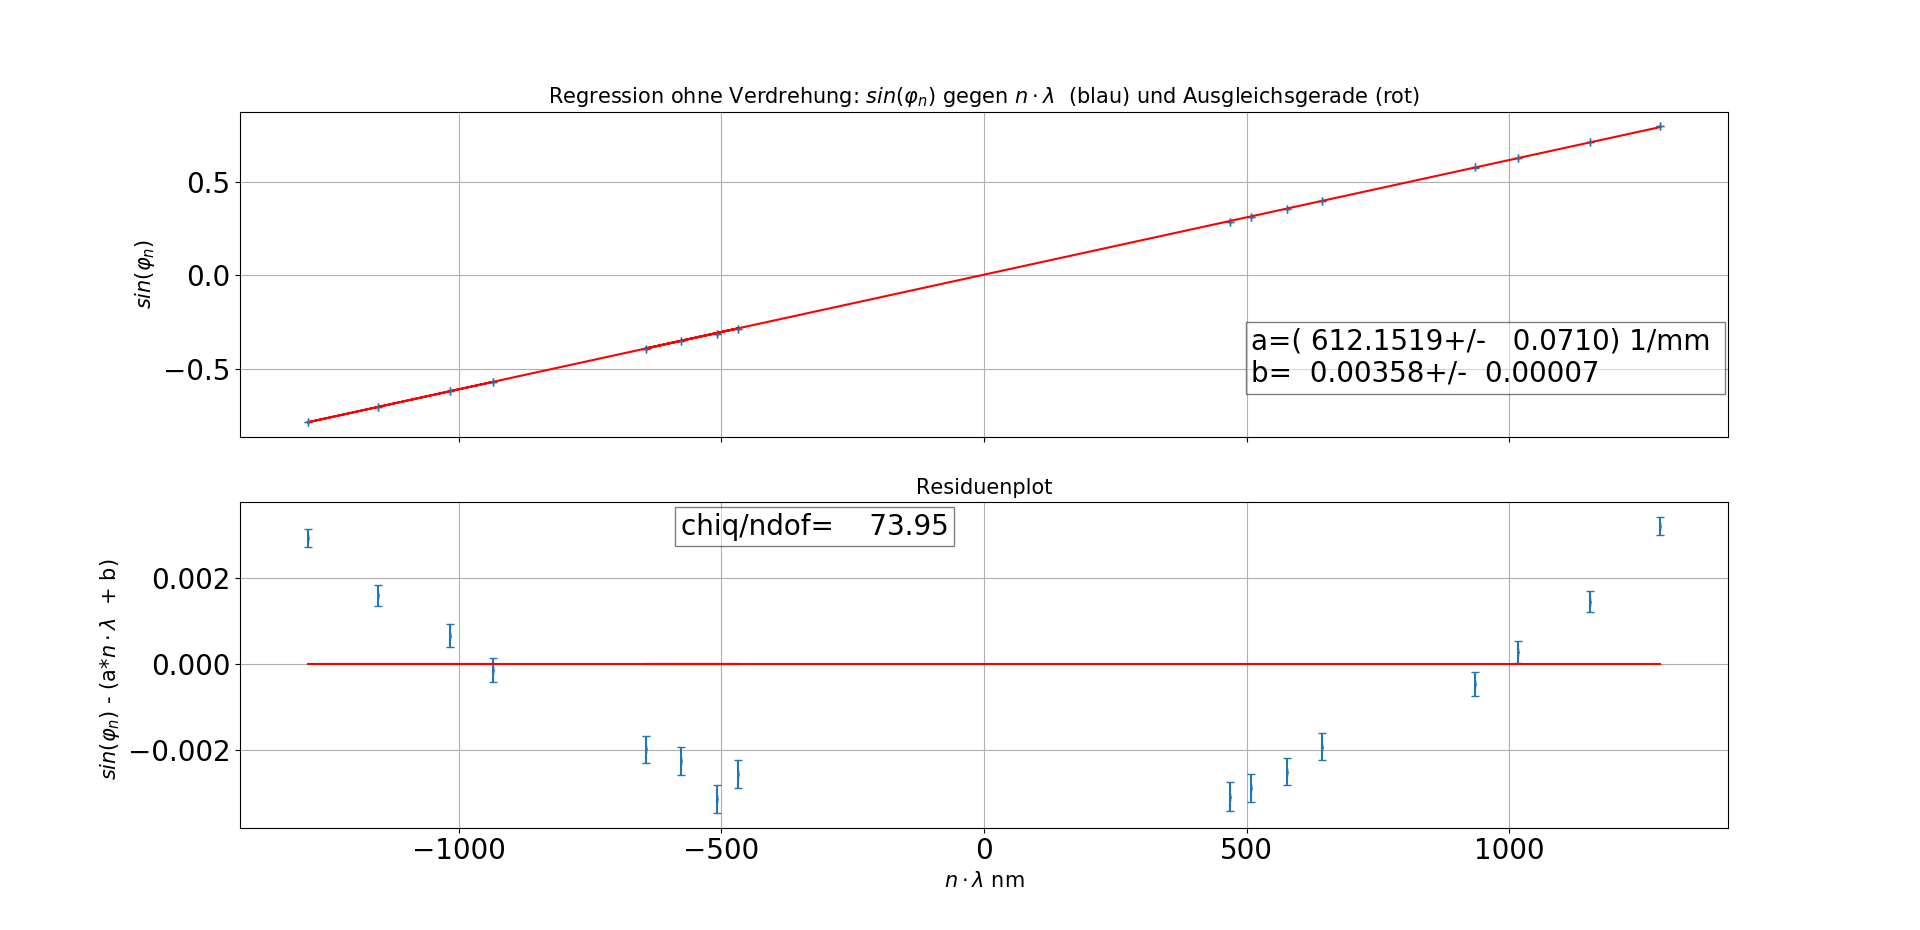
\includegraphics[scale=0.4]{./Bilder/Gitter_Regression_ohne_Verdrehung.png}
	\caption{Lineare Regression ohne Beachtung der Verdrehung des Gitter}
	\label{pic:linReg_1}	
\end{figure}

Aus der Steigung lässt sich dann die Gitterkonstante $g = \frac{1}{a}$ mit statistischer Unsicherheit $ \sigma_{g, stat} = \frac{\sigma_{a_{stat}}}{a^2}$ bestimmen (entsprechend für die systematische Unsicherheit).  

Die systematische Unsicherheit erhält man dabei aus der Verschiebemethode. Hier wurde dafür die Nulllinie jeweils um eine Standardabweichung in jede Richtung verschoben und die halbe Differenz der Steigungen als systematischer Fehler auf die Steigung der ursprünglichen linearen Regression verwendet (Tabelle \ref{table: aSys})
\begin{table}[H]
	\renewcommand{\arraystretch}{1.5}
	\large
	\centering
	\begin{tabular}{|c|c|}
		\hline
		$a_+$	&	$(612.1530 \pm 0.0710) \frac{1}{mm}$ \\
		\hline
		$a_-$	&	$(612.1508 \pm 0.0710) \frac{1}{mm}$ \\
		\hline
		$\sigma_{a_{sys}} = \frac{a_+ - a_-}{2}$	&	$ 0.011 \frac{1}{mm} $ \\
		\hline
		$b_+$	&	$0.00343 \pm 0.00007$ \\
		\hline
		$b_-$	&	$0.00372 \pm 0.00007$ \\
		\hline
		$\sigma_{b_{sys}} = \frac{b_+ - b_-}{2}$	&	$ 0.00015 $ \\
		\hline
	\end{tabular}
	\caption{Steigungen der um $\pm \sigma_{\varphi_0}$ verschobenen linearen Regressionen, siehe Abbildungen \ref{pic:linReg_1_+}, \ref{pic:linReg_1_-}}
	\label{table: aSys}
\end{table}
Die Ergebnisse der linearen Regression, sowie die berechnete Gitterkonstante sind in Tabelle \ref{table: linReg_final} jeweils in der Form $Wert \pm \sigma_{stat} \pm \sigma_{sys}$ zusammengefasst.

\begin{table}[H]
	\renewcommand{\arraystretch}{1.5}
	\large
	\centering
	\begin{tabular}{|c|c|}
		\hline
		$a$ &	$(612.1519 \pm 0.0710 \pm 0.0011) \frac{1}{mm}$ \\
		\hline
		$b$	&	$(0.00358 \pm 0.00007 \pm 0.00015) $ \\
		\hline
		$\frac{\chi^2}{ndof}$	&	$73.95$ \\
		\hline
		$g$	&	$(1633.582 \pm 0.190 \pm 0.003) \,nm$ \\
		\hline
		Abweichung vom Realwert $\frac{1 \,mm}{600} \approx	1666.7\, nm$	&	$ 174.50\sigma $ \\
		\hline
		relative Abweichung $1 - \frac{g_{gemessen}}{g_{real}}$ &	$ 1.99 \%$ \\
		\hline
	\end{tabular}
	\caption{Ergebnisse der linearen Regression}
	\label{table: linReg_final}
\end{table}

Eine der hier noch nicht beachteten Systematiken ist die Verdrehung des Gitters gegenüber der Einfallsrichtung des Lichtes. Dass dies bei der Auswertung eine Rolle spielt erkennt man deutlich am Residuum der linearen Regression, da diese eine Wannenform aufweist (siehe \ref{pic:linReg_1}). 

\paragraph{Korrektur der Gitterverdrehung}
Um diesen Fehler zu korrigieren wird eine erneute Anpassung durchgeführt, diesmal betrachtet man jedoch die obige Formel in der korrigierten Form 
\begin{equation}
\frac{1}{g} \cdot n \cdot \lambda = sin(\vartheta) + sin(\varphi_n - \vartheta)
\end{equation}
mit dem Verdrehungswinkel $\vartheta$. Um gleichzeitig die Steigung $\tilde{a}$ und den Ordinaten-Abschnitt $\tilde{b}$ der linearen Regression
\begin{equation}
\tilde{a} \cdot n \cdot \lambda + \tilde{b} = sin(\vartheta) + sin(\varphi_n - \vartheta)
\end{equation}
sowie den Verdrehungswinkel $\vartheta$ zu bestimmen, wird die Methode der Intervallschachtelung für $\vartheta$ angewandt und dabei versucht das $\frac{\chi^2}{ndof}$ zu minimieren.

Dabei wird ein fest vorgegebenes Winkelintervall (hier $\left[ -\frac{\pi}{6}, +\frac{\pi}{6}\right]$), in dem $\vartheta$ liegt immer weiter verkleinert, indem man jeweils für einen Wert in der rechten Intervallhälfte und für einen in der Linken eine lineare Regression durchführt und die $\frac{\chi^2}{ndof}$ miteinander vergleicht. Dieses verfahren wird dann rekursiv in dem Teilintervall durchgeführt, welches das kleinere $\frac{\chi^2}{ndof}$ liefert, bis man entweder 20 Durchläufe erreicht, oder sich der berechnete Winkel (bis auf ein Epsilon) nicht mehr ändert.
Abbildung \ref{pic:linReg_2} zeigt die finale lineare Regression.

\begin{figure}[H]
	\hskip-2cm
	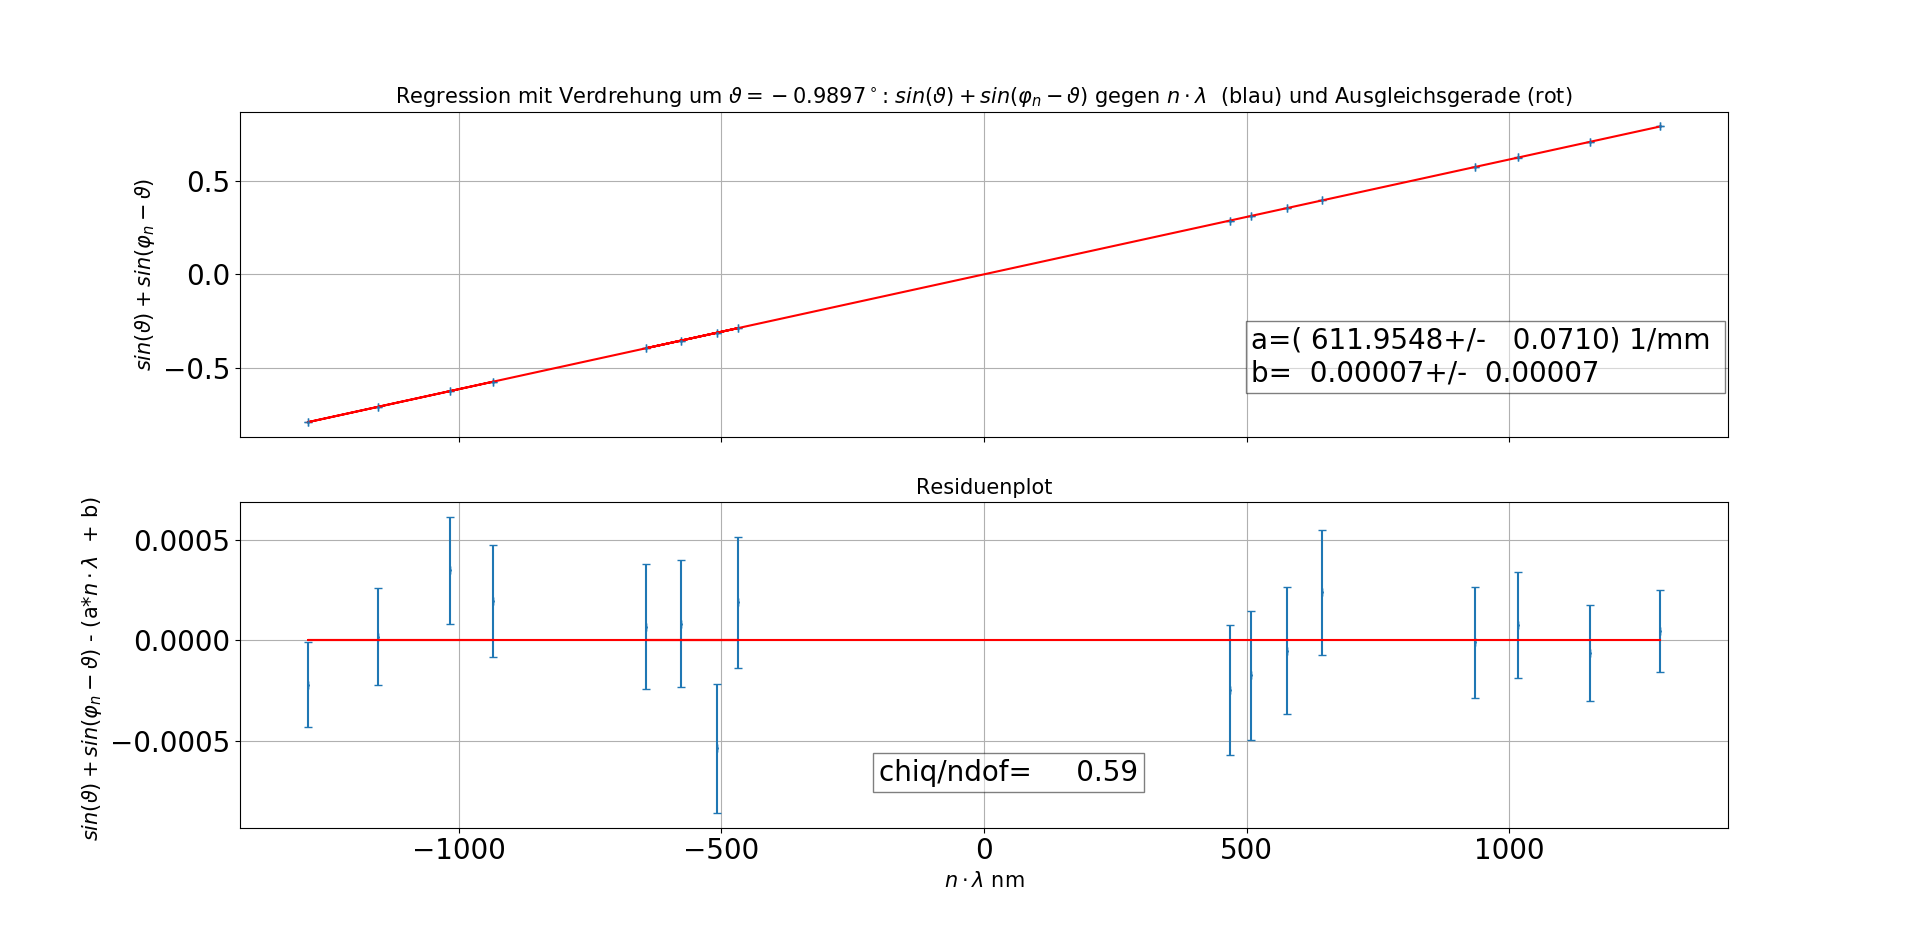
\includegraphics[scale=0.4]{./Bilder/Gitter_Regression_mit_Verdrehung.png}
	\caption{Lineare Regression mit Beachtung der Verdrehung des Gitters}
	\label{pic:linReg_2}	
\end{figure}

Die Unsicherheiten auf die Steigung und den Achsenabschnitt ergeben sich dabei analog zur Anpassung ohne Beachtung der Verdrehung. Für die systematischen Unsicherheiten siehe Tabelle \ref{table: aSys_2}.

\begin{table}[H]
	\renewcommand{\arraystretch}{1.5}
	\large
	\centering
	\begin{tabular}{|c|c|}
		\hline
		$\tilde{a}_+$	&	$(611.9579 \pm 0.0710) \frac{1}{mm}$ \\
		\hline
		$\tilde{a}_-$	&	$(611.9517 \pm 0.0710) \frac{1}{mm}$ \\
		\hline
		$\sigma_{\tilde{a}_{sys}} = \frac{\tilde{a}_+ - \tilde{a}_-}{2}$	&	$ 0.031 \frac{1}{mm} $ \\
		\hline
		$\tilde{b}_+$	&	$-0.00008 \pm 0.00007$ \\
		\hline
		$\tilde{b}_-$	&	$0.00022 \pm 0.00007$ \\
		\hline
		$\sigma_{\tilde{b}_{sys}} = \frac{\tilde{b}_- - \tilde{b}_+}{2}$	&	$ 0.00015 $ \\
		\hline
	\end{tabular}
	\caption{Steigungen der um $\pm \sigma_{\varphi_0}$ verschobenen linearen Regressionen unter Beachtung der Verdrehung des Gitters, siehe Abbildungen \ref{pic:linReg_2_+}, \ref{pic:linReg_2_-}}
	\label{table: aSys_2}
\end{table}

Theoretisch ließe sich der Verdrehungswinkel mit der oben beschriebenen Methode beliebig genau bestimmen. Allerdins sind die Messung der anderen Winkel fehlerbehaftet, was sich wiederum auf das Ergebnis für den Verdrehungswinkel auswirkt. Daher wird auch diese Unsicherheit mit der Verschiebungsmethode bestimmt. Hier wurden jedoch die Winkel um den kombinierten statistischen Fehler der Winkelmessung und den der Nulllinienmessung verschoben:
\begin{equation*}\label{eq:FehlerPhi}
\sigma_{\varphi} = \sqrt{\sigma_{\varphi_0}^2 + \sigma_{\varphi_n}^2}
\end{equation*}
Die Ergebnisse für die bestimmten Winkel $\vartheta$ sind in Tabelle \ref{table: theta} zusammengefasst.

\begin{table}[H]
	\renewcommand{\arraystretch}{1.5}
	\large
	\centering
	\begin{tabular}{|c|c|}
		\hline
		$\vartheta_+$	&	$ -0.9675^\circ $ \\
		\hline
		$\vartheta_-$	&	$ -1.0119^\circ $ \\
		\hline
		$\sigma_{\vartheta} = \frac{\vartheta_+ - \vartheta_-}{2}$	&	$ 0.0222 $ \\
		\hline
		$\vartheta$		&	$ -0.9897^\circ \pm 0.0222^\circ $	\\
		\hline
	\end{tabular}
	\caption{Verdrehungswinkel bei ursprünglicher Regression, sowie bei einer Verschiebung der Winkel um $\pm \sigma_{\varphi} = \pm \sqrt{\sigma_{\varphi_0}^2 + \sigma_{\varphi_n}^2} $}
	\label{table: theta}
\end{table}

Damit ergeben sich für die Steigung $\tilde{a}$ und den Ordinaten-Abschnitt $\tilde{b}$ der linearen Regression, sowie für die daraus berechnete Gitterkonstante die in Tabelle \ref{table: linReg_2_final} aufgeführten Ergebnisse.

\begin{table}[H]
	\renewcommand{\arraystretch}{1.5}
	\large
	\centering
	\begin{tabular}{|c|c|}
		\hline
		$\vartheta$		&	$ -0.9897^\circ \pm 0.0222^\circ $	\\
		\hline
		$\tilde{a}$ &	$(611.9548 \pm 0.0710 \pm 0.0031) \frac{1}{mm}$ \\
		\hline
		$\tilde{b}$	&	$(0.000068 \pm 0.000069 \pm 0.000148) $ \\
		\hline
		$\frac{\chi^2}{ndof}$	&	$0.59$	\\
		\hline
		$\tilde{g}$	&	$(1634.108 \pm 0.190 \pm 0.008)\, nm$ \\
		\hline
		Abweichung vom Realwert $\frac{1 \,mm}{600} \approx	1666.7\, nm$	&	$ 171.47 $ \\
		\hline
		relative Abweichung $1 - \frac{\tilde{g}_{gemessen}}{g_{real}}$ &	$ 1.96 \%$ \\
		\hline
	\end{tabular}
	\caption{Ergebnisse der linearen Regression, nach Korrektur um Verdrehugswinkel des Gitters}
	\label{table: linReg_2_final}
\end{table}
Ein Vergleich mit den Ergebnissen aus Tabelle \ref{table: linReg_final} zeigt, dass sich die Ergebnisse nicht bedeutend ändern, sowohl die Abweichung in Standardabweichungen, als auch die relative Abweichung bleiben in der selben Größenordnung. Lediglich das $\frac{\chi^2}{ndof}$ verringert sich merklich und das resultierende Residuum des Fits in Abbildung \ref{pic:linReg_2} zeigt keinerlei Systematiken mehr.


\subsubsection{Bestimmung der Wellenlängen der \texttt{Na}-Doppellinie}
\begin{figure}[H]
	\centering
	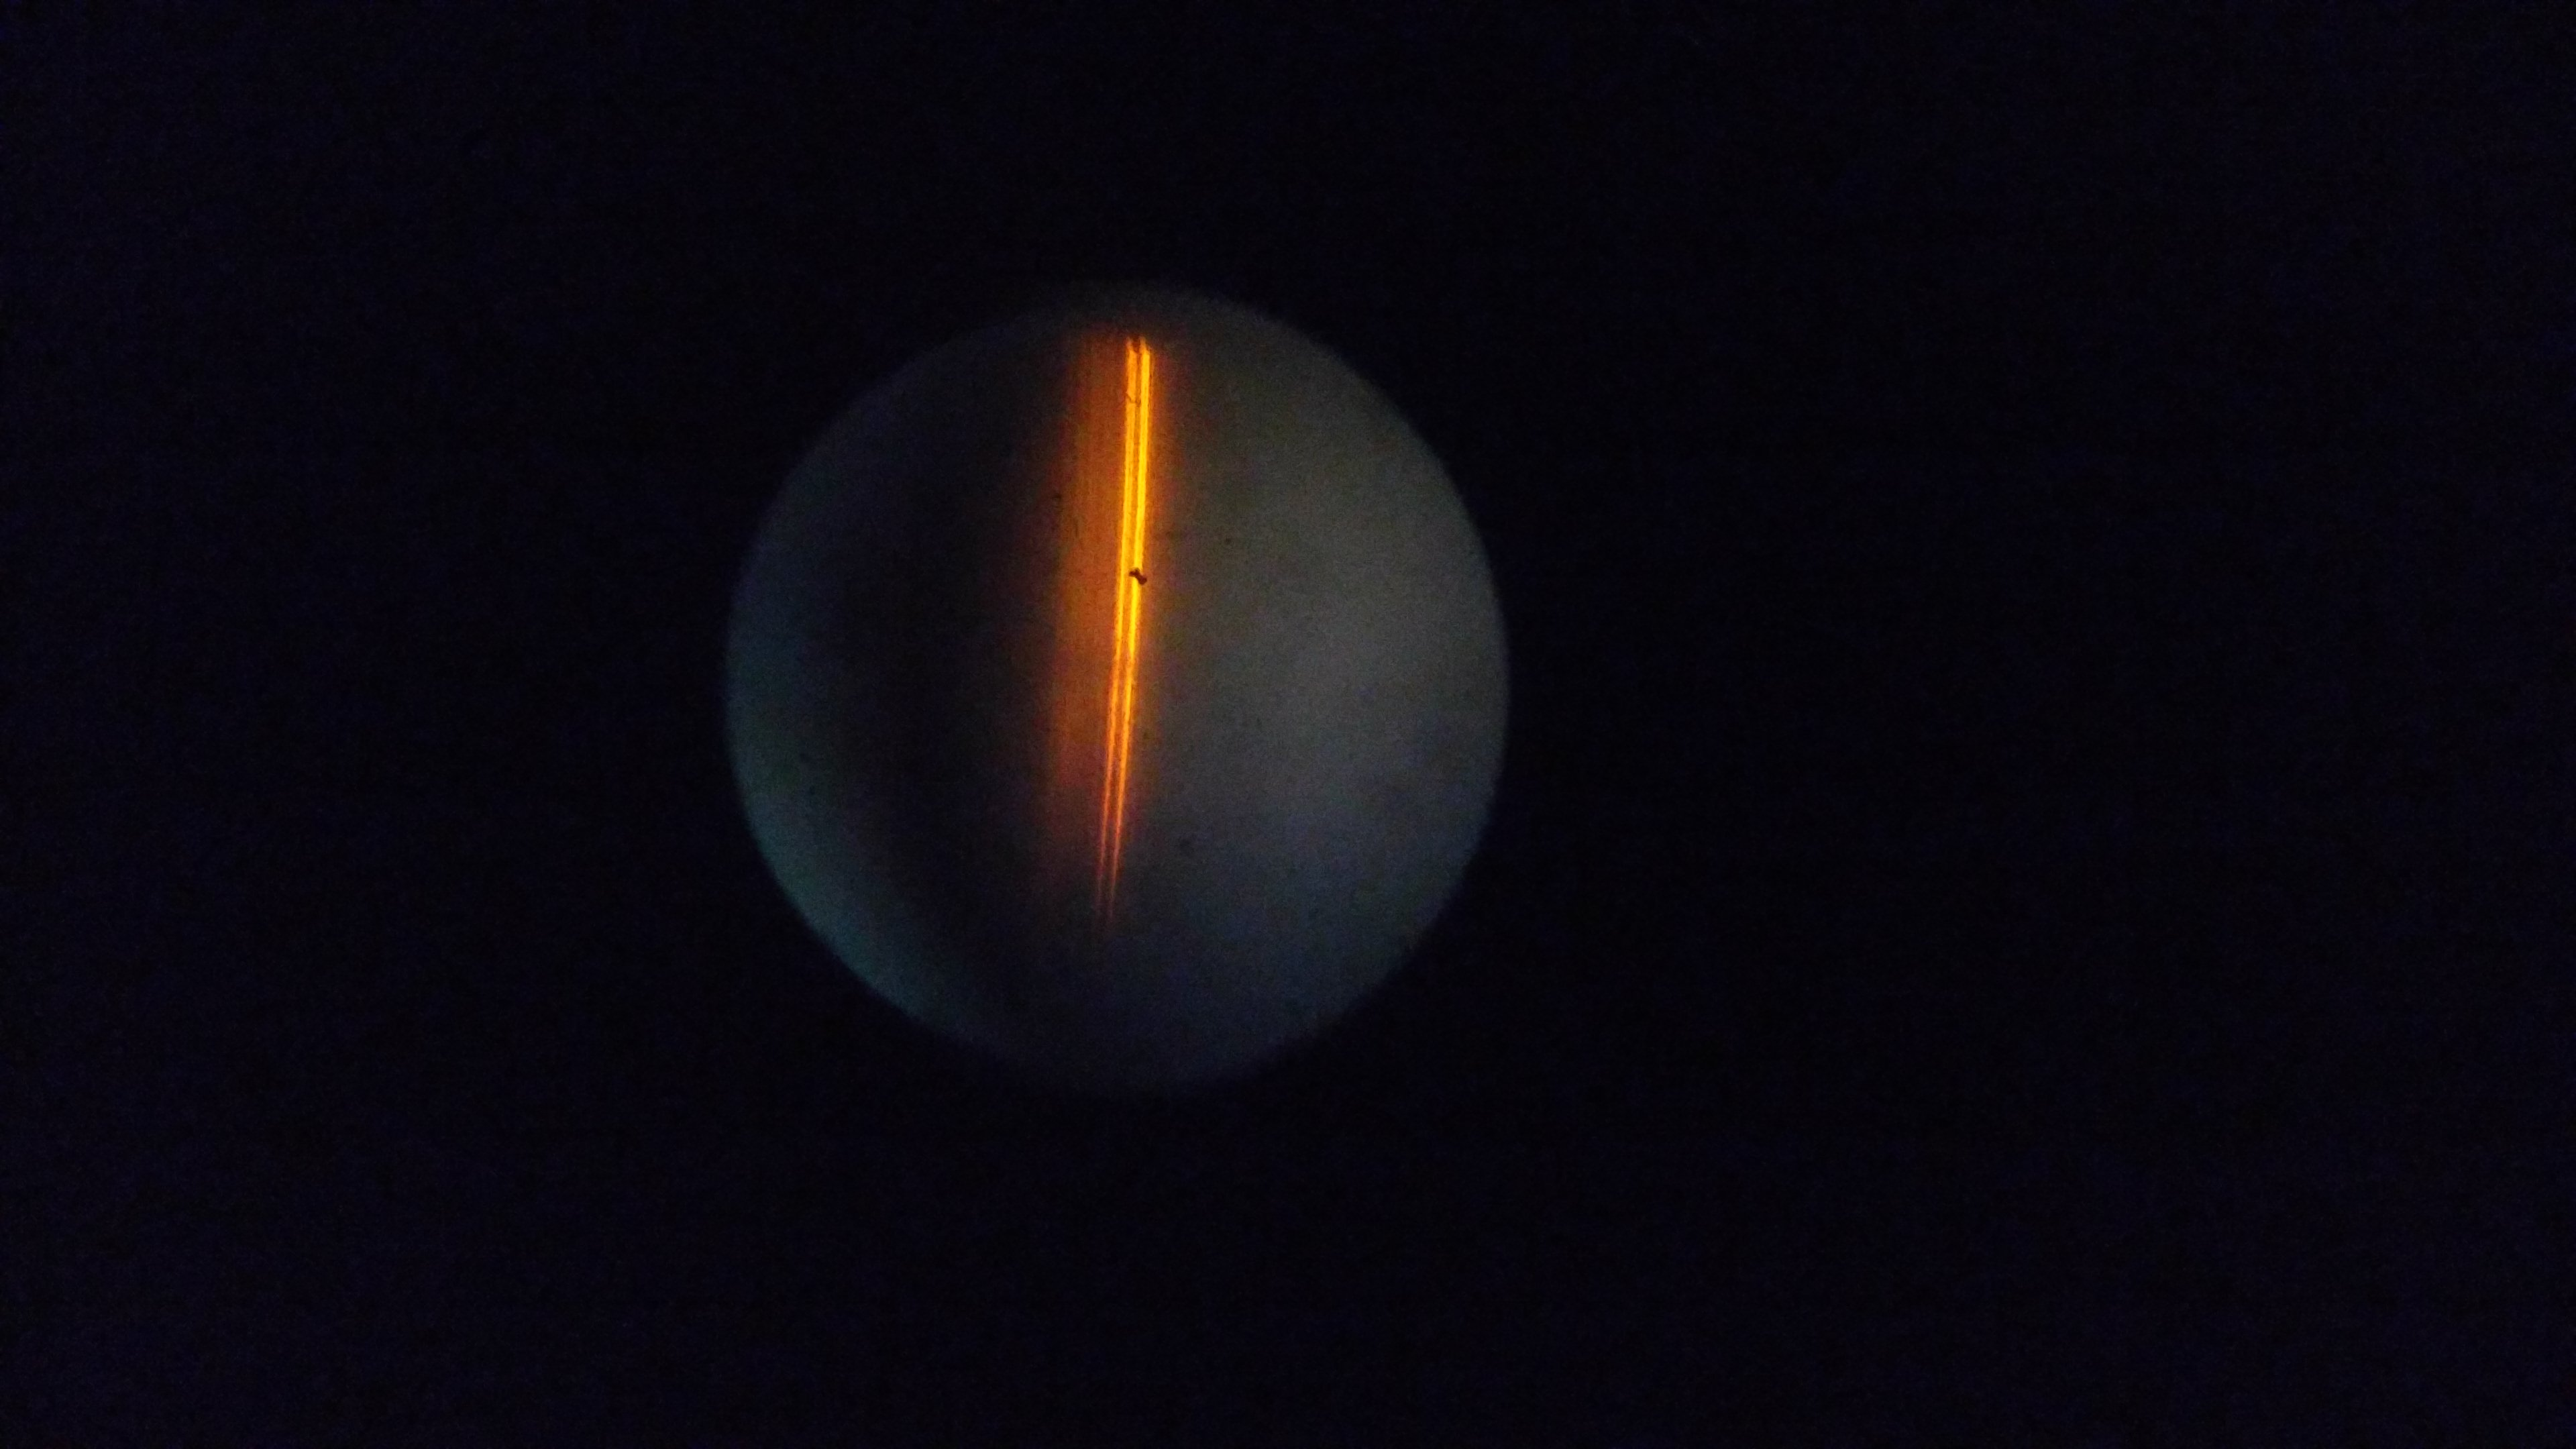
\includegraphics[trim={20cm 10cm 30cm 10cm},clip=true,scale=0.1]{./Bilder/IMG_20170915_130348.jpg}
	\caption{\texttt{Na}-Doppellinie sichtbar durch das Fernrohr}
	\label{pic:NaDoppellinie}
\end{figure}


Mit der nun bestimmten Gitterkonstante und Verdrehung des Gitters (Tabelle \ref{table: linReg_2_final}) kann aus der Messung der \texttt{Na}-Doppellinie dessen Wellenlänge bestimmt werden. Aus Gleichung \ref{eq:GitterVerdreht} folgt für den Fehler auf die berechnete Wellenlänge:
\begin{eqnarray*}\label{eq:LambdaFehler}
& \lambda = \frac{g}{n} \cdot ( \sin{\vartheta} + \sin(\varphi_n - \vartheta) )
\\
& \Rightarrow \sigma_\lambda = \frac{1}{|n|} \cdot \sqrt{ \left(\sin(\vartheta)+\sin(\varphi_n-\vartheta)\right)^2 \sigma_g^2 + g^2\left(\cos(\vartheta)-\cos(\varphi_n-\vartheta)\right)^2 \sigma_\vartheta^2 + g^2 \cos(\varphi_n-\vartheta)^2 \sigma_{\varphi_n}^2     }
\end{eqnarray*}
wobei wie zuvor $\sigma_{\varphi_n} = \sqrt{\sigma_{\varphi_0}^2+\sigma_{\varphi_{n,gemessen}}^2}$ gilt (siehe \ref{Bestimmung der Beugungswinkel}).
Für die \texttt{Na}-Doppellinie wurden folgende Werte ermittelt:

\begin{table}[H]
	\large
	\centering
	\begin{tabular}{|c|c|c|c|c|}
		\hline 
		Linie & -2. Ordnung $[nm]$  &   -1. Ordnung $[nm]$ &   1.Ordnung $[nm]$    &   2. Ordnung $[nm]$ \\
		\hline
		gelb (1) &   $588.889 \pm 0.252$   &   $588.635 \pm 0.600$    &   $588.011 \pm 0.592$    &   $588.435 \pm 0.247$ \\
		\hline
		gelb (2)  &   $589.677 \pm 0.252$   &   $589.676 \pm 0.599$    &   $589.331 \pm 0.592$    &   $589.023 \pm 0.247$ \\
		\hline
	\end{tabular}
	\caption{Nach Gleichung \ref{eq:LambdaFehler} berechnete Wellenlängen der Spektrallinien der \texttt{Na}-Lampe}
	\label{table:gemNaWellenlängen}
\end{table}

Die sich daraus ergebenden Wellenlängen der \texttt{Na}-Doppellinie sind in Tabelle \ref{table:NaWellenlängeErgebnisse} dargestellt.

\begin{table}[H]
	\large
	\centering
	\begin{tabular}{|c|c|c|c|}
		\hline
		Linie & \multicolumn{2}{|c|}{Wellenlänge $[nm]$} & Abweichung\\
		&	\texttt{NIST}-Wert & berechneter Wert & \\
		\hline
		gelb (1) & 589.59 & $588.61 \pm 0.16$ & $2.42\sigma$ \\
		\hline
		gelb (2) & 589.00 & $589.37 \pm 0.16$ & $1.37\sigma$ \\
		\hline
	\end{tabular}
	\caption{Bestimmte Wellenlänge der \texttt{Na}-Doppellinie mit Abweichung vom Realwert}
	\label{table:NaWellenlängeErgebnisse}
\end{table}

Mit dieser Methode konnten die Wellenlängen also mit geringem Fehler bestimmt werden, was aber auch zu einem relativ hohen Abweichung in Standardabweichunge führt.


\subsubsection{Bestimmung des Auflösungsvermögens}
Das minimal benötigte Auflösungsvermögen beträgt nach Formel \ref{eq:AGitter}
\begin{equation*}
A_{min} = \frac{\lambda}{\Delta \lambda} = \frac{589.00nm}{0.59nm} \approx 998.31
\end{equation*}

Die mit Hilfe der Schlitzblende bestimmten Auflösungsvermögen für die einzelnen Ordnungen sind in Tabelle \ref{table:Auflösungsvermögen} zu sehen. Dabei konnte die \texttt{Na}-Doppellinie für die beiden ersten Ordnungen beim Wechsel der Blende $d$ von $2mm$ zu $1.5mm$, und für die beiden zweiten Ordnungen von $1mm$ zu $0.5mm$ nicht mehr aufgelöst werden. Daher wurde jeweils die Mitte des Intervalls genommen, wobei sich der Fehler aus der Gleichverteilung mit $\sigma_d=0.5mm/\sqrt{12}$ ergab. Daraus wurde das Auflösungsvermögen wie folgt berechnet:
\begin{equation}
A = n \cdot \frac{d}{g}, \qquad \sigma_A = |n| \cdot \sqrt{\left(\frac{\sigma_d}{g}\right)^2 + \left(\frac{d}{g^2}\right)^2 \sigma_g^2}
\end{equation}
mit der Gitterkonstante $g$ und $\sigma_g$ aus Tabelle \ref{table: linReg_2_final}.

\begin{table}[H]
	\large
	\centering
	\begin{tabular}{|c|c|c|c|c|}
		\hline 
		& -2. Ordnung  &   -1. Ordnung &   1.Ordnung    &   2. Ordnung \\
		\hline
		$A$ &   $917.93 \pm 176.66$   &   $1070.92 \pm 88.33$    &   $1070.92 \pm 88.33$    &   $1040.32 \pm 55.86$\\
		\hline
		$A_{Mittel}$  &   \multicolumn{4}{|c|}{$1040.32 \pm 55.86$} \\
		\hline
		$A_{min}$ & \multicolumn{4}{|c|}{$998.31$} \\
		\hline
		Abweichung & \multicolumn{4}{|c|}{$0.75\sigma$} \\
		\hline
	\end{tabular}
	\caption{Bestimmte Auflösungsvermögen mit Abweichung}
	\label{table:Auflösungsvermögen}
\end{table}

Somit konnte das Auflösungsvermögen ungefähr ermittelt werden und liegt innerhalb von einer Standardabweichung vom theoretischen Wert.
Zu beachten ist allerdings, dass die Formel \ref{eq:AGitter} nur das für die \texttt{Na}-Doppellinie minimal benötigte Auflösungsvermögen angibt, und das Auflösungsvermögen des verwendeten Gitters durchaus dadrüber liegen kann.

%\clearpage
\subsection{Fazit}
\paragraph{Gitterkonstante}
Es fällt sofort auf, dass die Abweichung in Standardabweichungen mit $170.5\sigma$ sehr hoch ist. Dies könnte aus zu kleinen Fehlerabschätzungen resultieren. Zum Beispiel könnte es sein, dass die Unsicherheit auf die Winkelmessung doch nicht als konstant angenommen werden kann. Auch die Nichtbeachtung einiger Systematiken könnte diese Abweichung zur Folge haben. Da jedoch die relative Abweichung mit knapp 2 Prozent noch im Rahmen liegt, werden diese wohl keinen allzu großen Einfluss haben und die hohe Abweichung folgt wahrscheinlich eher aus den recht kleinen Unsicherheiten.

Da diese Ergebnisse (bis auf das $\chi^2/ndf$) sich auch nach Korrektur um den Drehwinkel nicht bedeutend ändert, lässt sich schließen dass entweder wie zuvor schon vermutet die Unsicherheiten auf die Winkelmessung nicht ideal abgeschätzt wurden, oder dass der Hersteller des Gitters weniger genau gearbeitet hat als angegeben.

\paragraph{Wellenlänge}
Die Fehler auf die bestimmten Wellenlängen waren alle relativ gering, wodurch eine relativ hohe Abweichung von $\sim2.5\sigma$ und $\sim 1.5\sigma$ vom Datenbankwert der \texttt{Na}-Doppellinie resultierte. Dies ist nicht allzu überraschend, da dieses Ergebnis von der zuvor ermittelten Gitterkonstante abhängt, die eine hohe Abweichung aufwies.

\paragraph{Auflösungsvermögen}
Trotz der nur schrittweise einstellbaren Blende und der daraus resultierenden relativ hohen Fehler lag das bestimmte Auflösungsvermögen innerhalb einer Standardabweichung vom theoretischen Wert. Zu beachten ist allerdings, dass die Formel \ref{eq:AGitter} nur das für die \texttt{Na}-Doppellinie minimal benötigte Auflösungsvermögen angibt, und das Auflösungsvermögen des verwendeten Gitters durchaus dadrüber liegen kann. \\
Zur genaueren Bestimmung würde sich hier eine variable Schlitzblende mit Feinstellschraube anbieten.


\clearpage
\section{Anhang}
\begin{figure}[H]
	\centering
	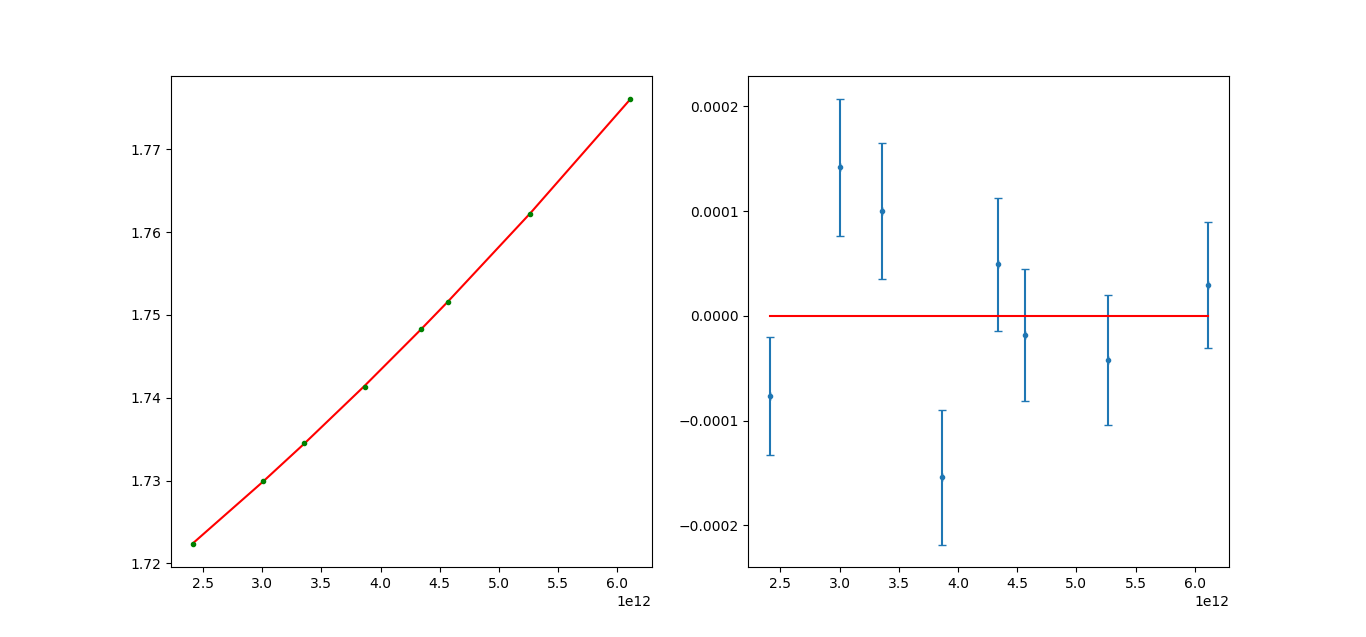
\includegraphics[trim = 0mm 0mm 0mm 0mm,clip, width=15cm]{Bilder/nicht_linearer_fit.png}%
	\caption[nicht linearer Fit]{nicht linearer Fit}%
	\label{pic:Abbildung 1}%
\end{figure}

\begin{figure}[H]
	\centering
	\hskip -2cm
	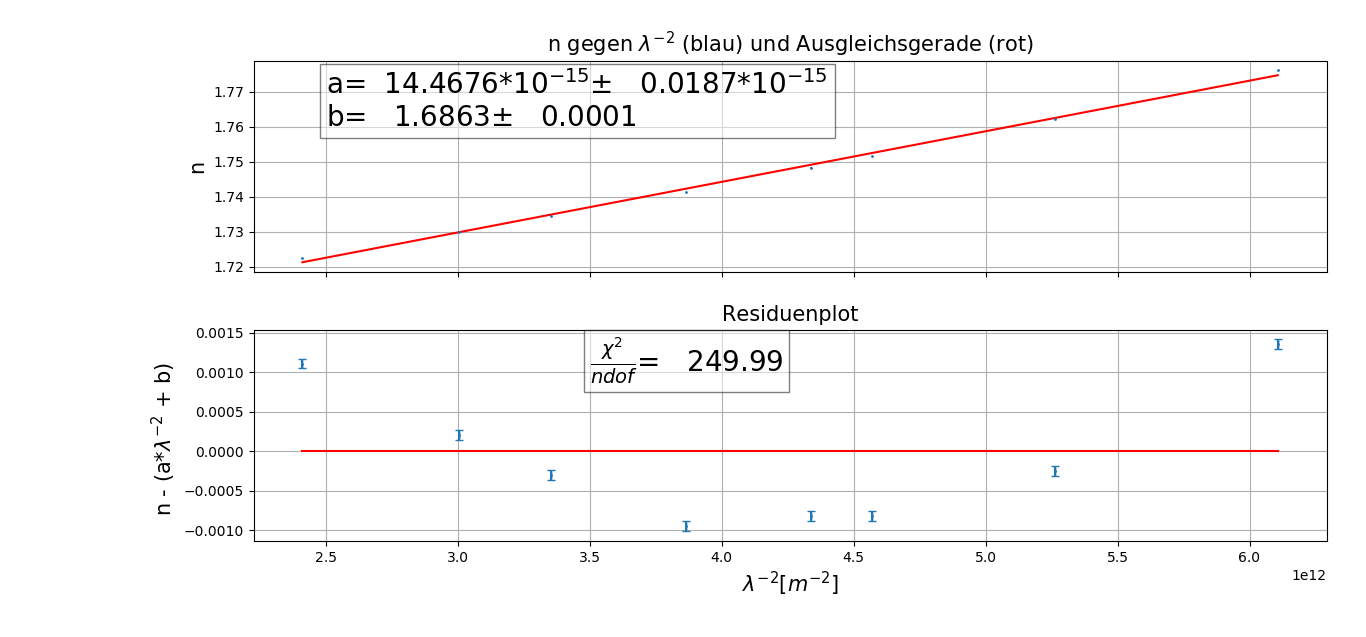
\includegraphics[trim = 0mm 0mm 0mm 0mm,clip,scale=0.5]{Bilder/lineare_fit.png}%
	\caption[lineare Regression]{lineare Regression}%
	\label{pic:Abbildung 1}%
\end{figure}

\begin{figure}[H]
	\hskip-2.5cm
	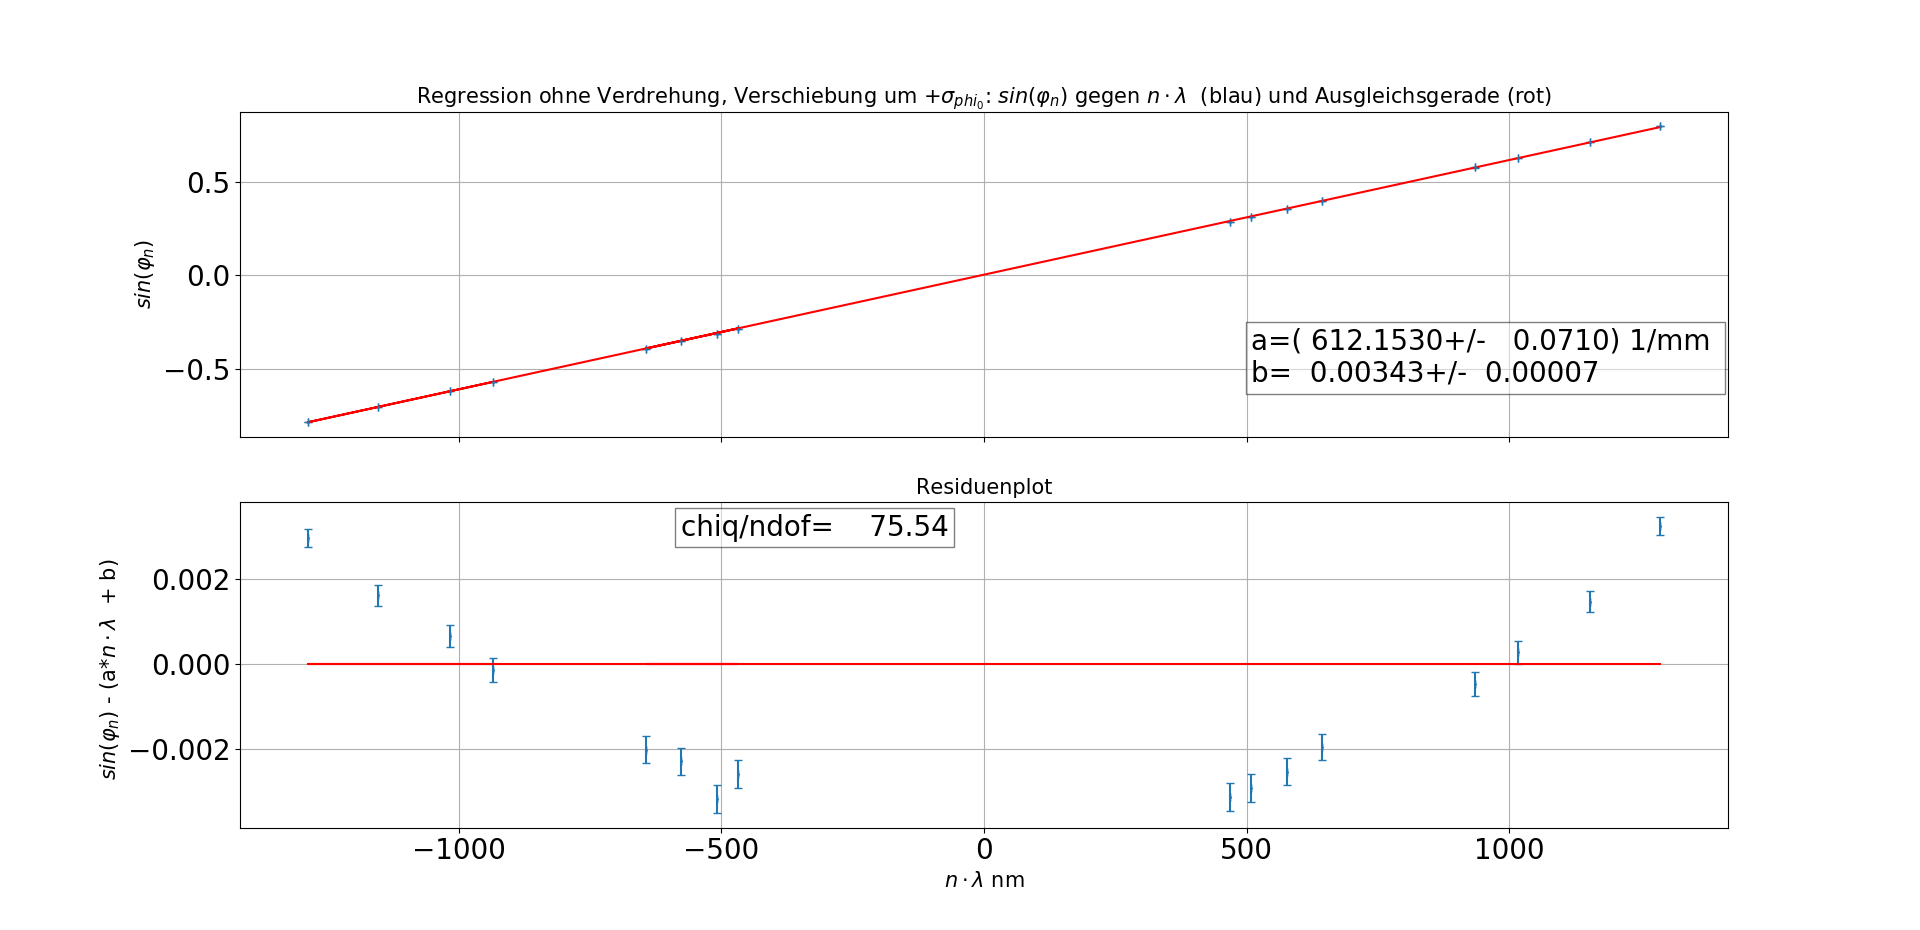
\includegraphics[scale=0.45]{./Bilder/Gitter_Regression_ohne_Verdrehung_+.png}
	\caption{lineare Regression ohne Beachtung der Verdrehung des Gitters, verschoben um $+ \sigma_{\varphi_0}$}
	\label{pic:linReg_1_+}	
\end{figure}

\begin{figure}[H]
	\hskip-2.5cm
	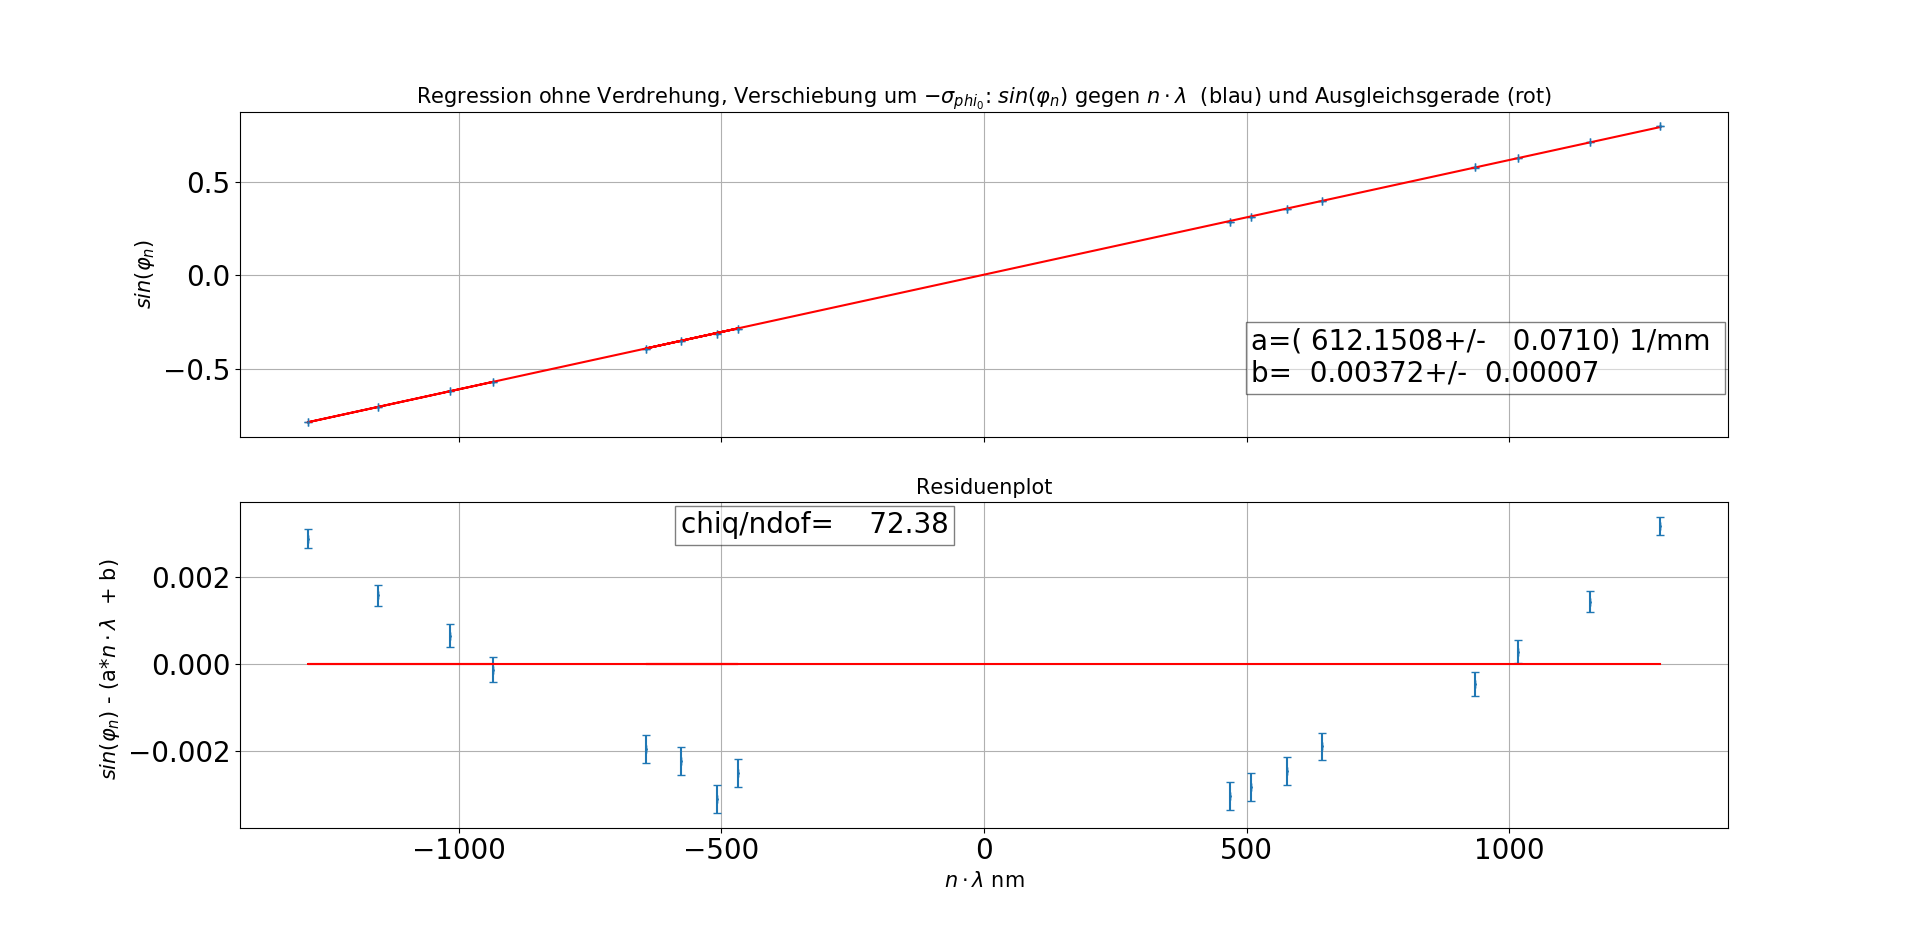
\includegraphics[scale=0.45]{./Bilder/Gitter_Regression_ohne_Verdrehung_-.png}
	\caption{lineare Regression ohne Beachtung der Verdrehung des Gitters, verschoben um $- \sigma_{\varphi_0}$}
	\label{pic:linReg_1_-}	
\end{figure}

\begin{figure}[H]
	\hskip-2.5cm
	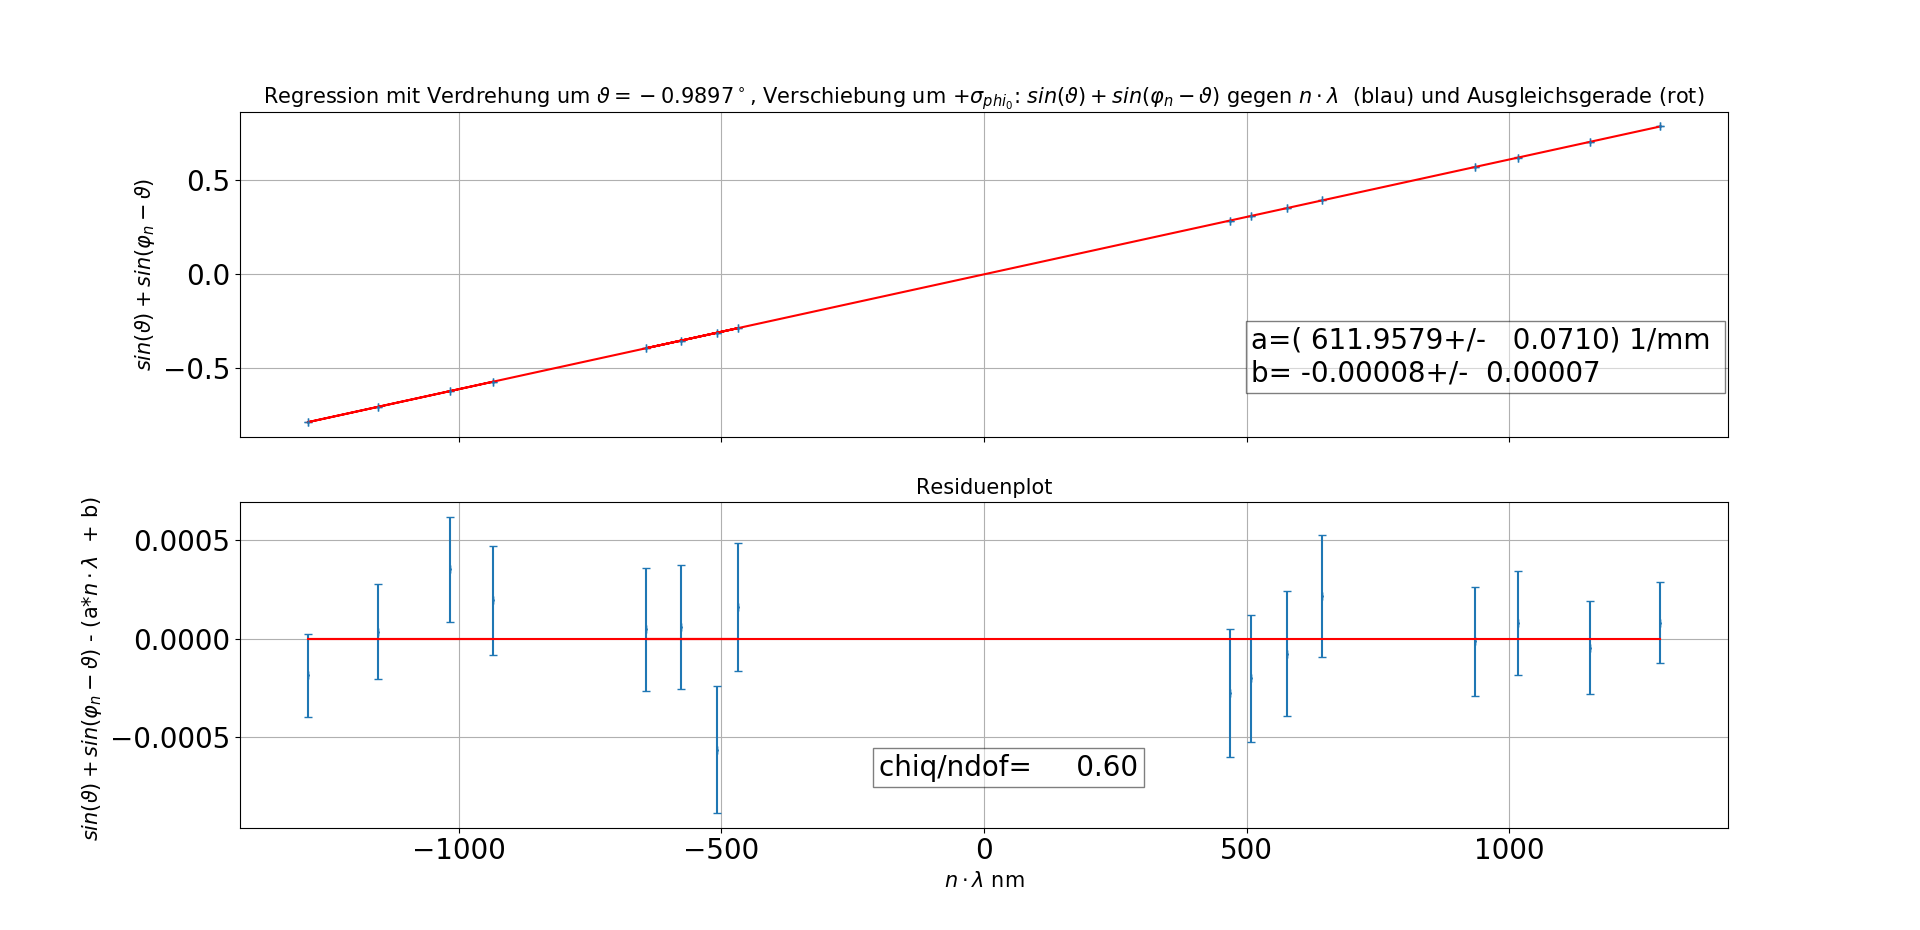
\includegraphics[scale=0.45]{./Bilder/Gitter_Regression_mit_Verdrehung_+.png}
	\caption{lineare Regression mit Beachtung der Verdrehung des Gitters, verschoben um $+ \sigma_{\varphi_0}$}
	\label{pic:linReg_2_+}	
\end{figure}

\begin{figure}[H]
	\hskip-2.5cm
	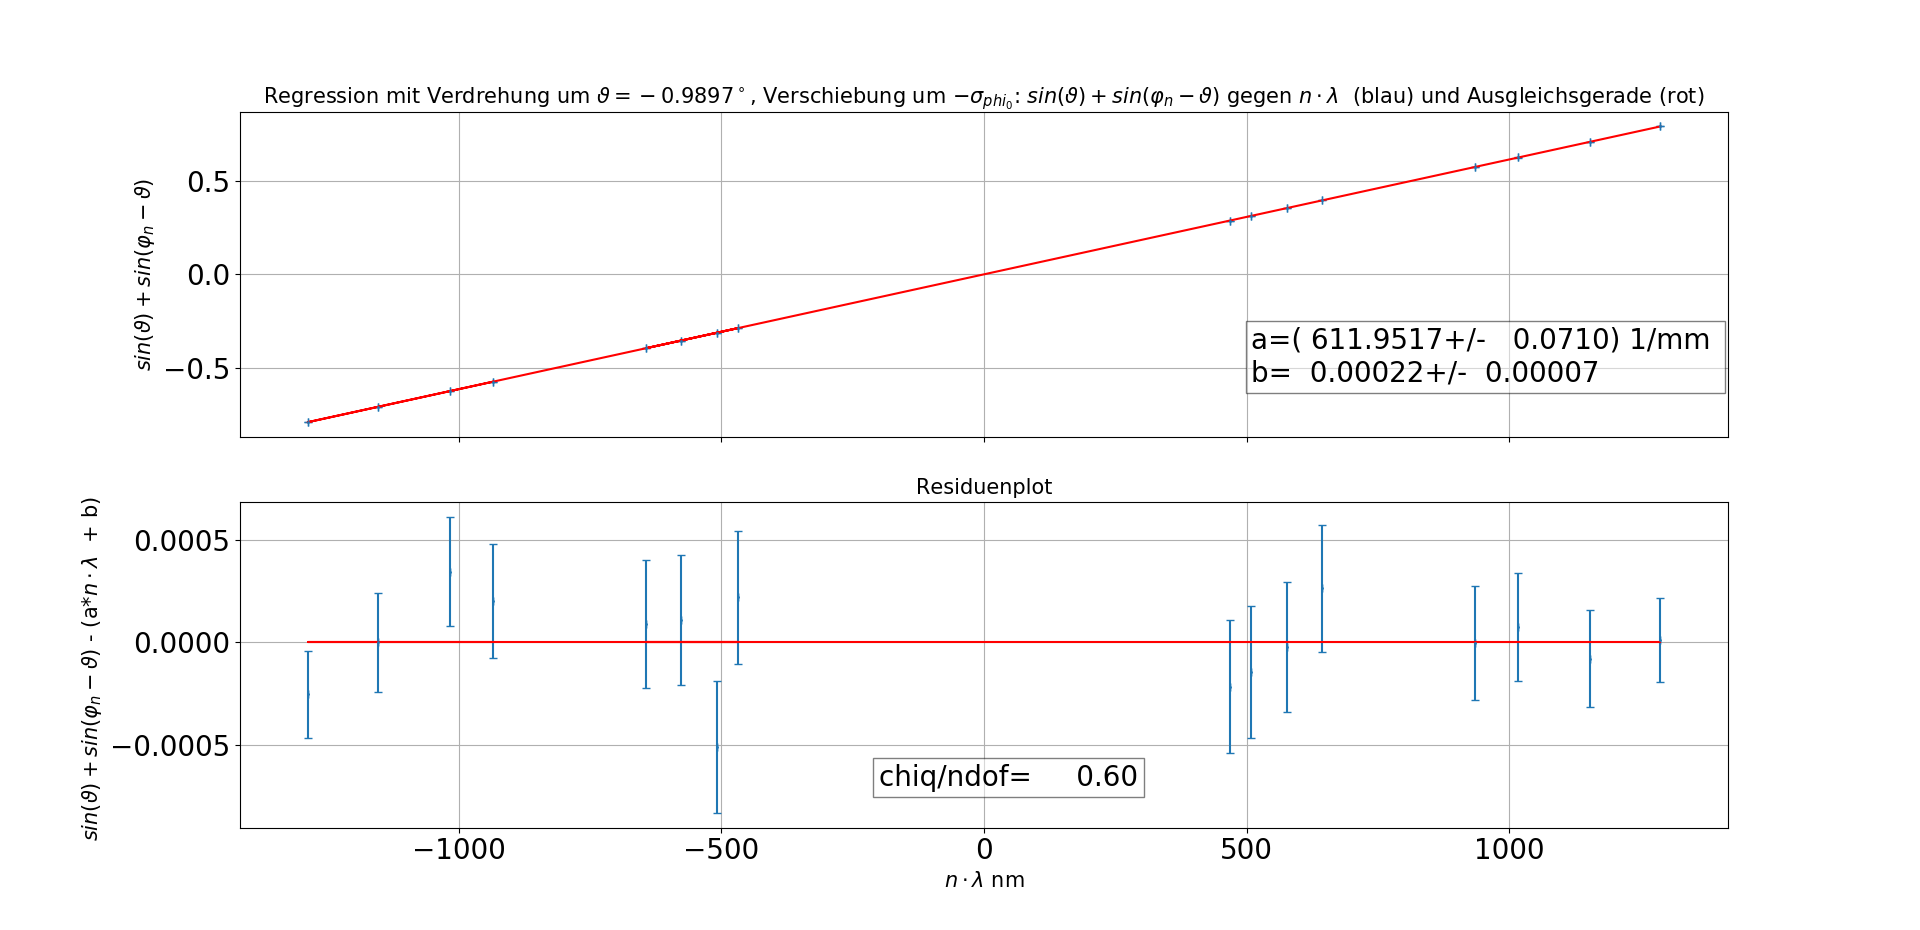
\includegraphics[scale=0.45]{./Bilder/Gitter_Regression_mit_Verdrehung_-.png}
	\caption{lineare Regression mit Beachtung der Verdrehung des Gitters, verschoben um $- \sigma_{\varphi_0}$}
	\label{pic:linReg_2_-}	
\end{figure}


\newpage
\listoffigures
\listoftables

\end{document}